% Options for packages loaded elsewhere
\PassOptionsToPackage{unicode}{hyperref}
\PassOptionsToPackage{hyphens}{url}
%
\documentclass[
]{article}
\usepackage{lmodern}
\usepackage{amssymb,amsmath}
\usepackage{ifxetex,ifluatex}
\ifnum 0\ifxetex 1\fi\ifluatex 1\fi=0 % if pdftex
  \usepackage[T1]{fontenc}
  \usepackage[utf8]{inputenc}
  \usepackage{textcomp} % provide euro and other symbols
\else % if luatex or xetex
  \usepackage{unicode-math}
  \defaultfontfeatures{Scale=MatchLowercase}
  \defaultfontfeatures[\rmfamily]{Ligatures=TeX,Scale=1}
\fi
% Use upquote if available, for straight quotes in verbatim environments
\IfFileExists{upquote.sty}{\usepackage{upquote}}{}
\IfFileExists{microtype.sty}{% use microtype if available
  \usepackage[]{microtype}
  \UseMicrotypeSet[protrusion]{basicmath} % disable protrusion for tt fonts
}{}
\makeatletter
\@ifundefined{KOMAClassName}{% if non-KOMA class
  \IfFileExists{parskip.sty}{%
    \usepackage{parskip}
  }{% else
    \setlength{\parindent}{0pt}
    \setlength{\parskip}{6pt plus 2pt minus 1pt}}
}{% if KOMA class
  \KOMAoptions{parskip=half}}
\makeatother
\usepackage{xcolor}
\IfFileExists{xurl.sty}{\usepackage{xurl}}{} % add URL line breaks if available
\IfFileExists{bookmark.sty}{\usepackage{bookmark}}{\usepackage{hyperref}}
\hypersetup{
  pdftitle={Tarea 1\_Modulo2},
  pdfauthor={Luisa María Acosta O.; Sebastian Agudelo J.; Laura Camila Agudelo O.; Karen Andrea Amaya M.; Estefania Echeverry F.},
  hidelinks,
  pdfcreator={LaTeX via pandoc}}
\urlstyle{same} % disable monospaced font for URLs
\usepackage[margin=1in]{geometry}
\usepackage{color}
\usepackage{fancyvrb}
\newcommand{\VerbBar}{|}
\newcommand{\VERB}{\Verb[commandchars=\\\{\}]}
\DefineVerbatimEnvironment{Highlighting}{Verbatim}{commandchars=\\\{\}}
% Add ',fontsize=\small' for more characters per line
\usepackage{framed}
\definecolor{shadecolor}{RGB}{248,248,248}
\newenvironment{Shaded}{\begin{snugshade}}{\end{snugshade}}
\newcommand{\AlertTok}[1]{\textcolor[rgb]{0.94,0.16,0.16}{#1}}
\newcommand{\AnnotationTok}[1]{\textcolor[rgb]{0.56,0.35,0.01}{\textbf{\textit{#1}}}}
\newcommand{\AttributeTok}[1]{\textcolor[rgb]{0.77,0.63,0.00}{#1}}
\newcommand{\BaseNTok}[1]{\textcolor[rgb]{0.00,0.00,0.81}{#1}}
\newcommand{\BuiltInTok}[1]{#1}
\newcommand{\CharTok}[1]{\textcolor[rgb]{0.31,0.60,0.02}{#1}}
\newcommand{\CommentTok}[1]{\textcolor[rgb]{0.56,0.35,0.01}{\textit{#1}}}
\newcommand{\CommentVarTok}[1]{\textcolor[rgb]{0.56,0.35,0.01}{\textbf{\textit{#1}}}}
\newcommand{\ConstantTok}[1]{\textcolor[rgb]{0.00,0.00,0.00}{#1}}
\newcommand{\ControlFlowTok}[1]{\textcolor[rgb]{0.13,0.29,0.53}{\textbf{#1}}}
\newcommand{\DataTypeTok}[1]{\textcolor[rgb]{0.13,0.29,0.53}{#1}}
\newcommand{\DecValTok}[1]{\textcolor[rgb]{0.00,0.00,0.81}{#1}}
\newcommand{\DocumentationTok}[1]{\textcolor[rgb]{0.56,0.35,0.01}{\textbf{\textit{#1}}}}
\newcommand{\ErrorTok}[1]{\textcolor[rgb]{0.64,0.00,0.00}{\textbf{#1}}}
\newcommand{\ExtensionTok}[1]{#1}
\newcommand{\FloatTok}[1]{\textcolor[rgb]{0.00,0.00,0.81}{#1}}
\newcommand{\FunctionTok}[1]{\textcolor[rgb]{0.00,0.00,0.00}{#1}}
\newcommand{\ImportTok}[1]{#1}
\newcommand{\InformationTok}[1]{\textcolor[rgb]{0.56,0.35,0.01}{\textbf{\textit{#1}}}}
\newcommand{\KeywordTok}[1]{\textcolor[rgb]{0.13,0.29,0.53}{\textbf{#1}}}
\newcommand{\NormalTok}[1]{#1}
\newcommand{\OperatorTok}[1]{\textcolor[rgb]{0.81,0.36,0.00}{\textbf{#1}}}
\newcommand{\OtherTok}[1]{\textcolor[rgb]{0.56,0.35,0.01}{#1}}
\newcommand{\PreprocessorTok}[1]{\textcolor[rgb]{0.56,0.35,0.01}{\textit{#1}}}
\newcommand{\RegionMarkerTok}[1]{#1}
\newcommand{\SpecialCharTok}[1]{\textcolor[rgb]{0.00,0.00,0.00}{#1}}
\newcommand{\SpecialStringTok}[1]{\textcolor[rgb]{0.31,0.60,0.02}{#1}}
\newcommand{\StringTok}[1]{\textcolor[rgb]{0.31,0.60,0.02}{#1}}
\newcommand{\VariableTok}[1]{\textcolor[rgb]{0.00,0.00,0.00}{#1}}
\newcommand{\VerbatimStringTok}[1]{\textcolor[rgb]{0.31,0.60,0.02}{#1}}
\newcommand{\WarningTok}[1]{\textcolor[rgb]{0.56,0.35,0.01}{\textbf{\textit{#1}}}}
\usepackage{graphicx,grffile}
\makeatletter
\def\maxwidth{\ifdim\Gin@nat@width>\linewidth\linewidth\else\Gin@nat@width\fi}
\def\maxheight{\ifdim\Gin@nat@height>\textheight\textheight\else\Gin@nat@height\fi}
\makeatother
% Scale images if necessary, so that they will not overflow the page
% margins by default, and it is still possible to overwrite the defaults
% using explicit options in \includegraphics[width, height, ...]{}
\setkeys{Gin}{width=\maxwidth,height=\maxheight,keepaspectratio}
% Set default figure placement to htbp
\makeatletter
\def\fps@figure{htbp}
\makeatother
\setlength{\emergencystretch}{3em} % prevent overfull lines
\providecommand{\tightlist}{%
  \setlength{\itemsep}{0pt}\setlength{\parskip}{0pt}}
\setcounter{secnumdepth}{-\maxdimen} % remove section numbering
\usepackage{booktabs}
\usepackage{longtable}
\usepackage{array}
\usepackage{multirow}
\usepackage{wrapfig}
\usepackage{float}
\usepackage{colortbl}
\usepackage{pdflscape}
\usepackage{tabu}
\usepackage{threeparttable}
\usepackage{threeparttablex}
\usepackage[normalem]{ulem}
\usepackage{makecell}

\title{\textbf{Tarea 1\_Modulo2}}
\author{\textbf{Luisa María Acosta O.} \and \textbf{Sebastian Agudelo J.} \and \textbf{Laura Camila Agudelo O.} \and \textbf{Karen Andrea Amaya M.} \and \textbf{Estefania Echeverry F.}}
\date{\textbf{Octubre 2020}}

\begin{document}
\maketitle

\textbf{Librerías}

\begin{Shaded}
\begin{Highlighting}[]
\CommentTok{#Librerias}
\KeywordTok{library}\NormalTok{(kableExtra, }\DataTypeTok{warn.conflicts=}\NormalTok{F, }\DataTypeTok{quietly=}\NormalTok{T)}\CommentTok{#tablas}
\KeywordTok{library}\NormalTok{(Hmisc,}\DataTypeTok{warn.conflicts=}\NormalTok{F, }\DataTypeTok{quietly=}\NormalTok{T) }\CommentTok{#Rezagos}
\KeywordTok{library}\NormalTok{(class,}\DataTypeTok{warn.conflicts=}\NormalTok{F, }\DataTypeTok{quietly=}\NormalTok{T)}\CommentTok{#knn}
\KeywordTok{library}\NormalTok{(caret,}\DataTypeTok{warn.conflicts=}\NormalTok{F, }\DataTypeTok{quietly=}\NormalTok{T) }\CommentTok{#cv}
\KeywordTok{require}\NormalTok{(ISLR,}\DataTypeTok{warn.conflicts=}\NormalTok{F, }\DataTypeTok{quietly=}\NormalTok{T)}
\KeywordTok{require}\NormalTok{(glmnet,}\DataTypeTok{warn.conflicts=}\NormalTok{F, }\DataTypeTok{quietly=}\NormalTok{T) }
\end{Highlighting}
\end{Shaded}

\begin{verbatim}
## Loaded glmnet 4.0-2
\end{verbatim}

\begin{Shaded}
\begin{Highlighting}[]
\CommentTok{#Función para normalizar variables}
\NormalTok{normalize <-}\StringTok{ }\ControlFlowTok{function}\NormalTok{(x) \{}
\NormalTok{  norm <-}\StringTok{ }\NormalTok{((x }\OperatorTok{-}\StringTok{ }\KeywordTok{min}\NormalTok{(x))}\OperatorTok{/}\NormalTok{(}\KeywordTok{max}\NormalTok{(x) }\OperatorTok{-}\StringTok{ }\KeywordTok{min}\NormalTok{(x)))}
  \KeywordTok{return}\NormalTok{ (norm)}
\NormalTok{\}}
\end{Highlighting}
\end{Shaded}

\textbf{1.} Descargue de Yahoo Finance la base de datos de los precios
de cierre diarios de la acción que se le asignó a su grupo
\textbf{(Grupo 9, HP inc.)} en el periodo que va del 1 de enero de 2015
hasta el 31 de diciembre de 2019

\begin{Shaded}
\begin{Highlighting}[]
\NormalTok{datos<-}\StringTok{ }\KeywordTok{read.csv}\NormalTok{(}\StringTok{"HPQ.csv"}\NormalTok{)}
\NormalTok{datos}\OperatorTok{$}\NormalTok{Date <-}\StringTok{ }\KeywordTok{as.Date}\NormalTok{(datos}\OperatorTok{$}\NormalTok{Date, }\DataTypeTok{format =} \StringTok{"%Y-%m-%d"}\NormalTok{)}
\KeywordTok{head}\NormalTok{(datos, }\DecValTok{3}\NormalTok{) }\OperatorTok\StringTok{ }\KeywordTok{kbl}\NormalTok{() }\OperatorTok\StringTok{ }\KeywordTok{kable_styling}\NormalTok{()}
\end{Highlighting}
\end{Shaded}

\begin{table}[H]
\centering
\begin{tabular}[t]{l|r|r|r|r|r|r}
\hline
Date & Open & High & Low & Close & Adj.Close & Volume\\
\hline
2015-01-02 & 18.19255 & 18.38329 & 17.97457 & 18.27430 & 14.83616 & 21604400\\
\hline
2015-01-05 & 18.07448 & 18.20618 & 17.83379 & 17.97003 & 14.58914 & 23850900\\
\hline
2015-01-06 & 18.10627 & 18.26521 & 17.67484 & 17.83379 & 14.47853 & 26398600\\
\hline
\end{tabular}
\end{table}

En primer lugar hacemos un análisis exploratorio de los datos. A
continuación podemos ver que la base de datos tiene 1250 observaciones
con 7 variables, de las cuales 6 son de tipo factor y una de tipo fecha.

\begin{Shaded}
\begin{Highlighting}[]
\KeywordTok{str}\NormalTok{(datos)}
\end{Highlighting}
\end{Shaded}

\begin{verbatim}
## 'data.frame':    1257 obs. of  7 variables:
##  $ Date     : Date, format: "2015-01-02" "2015-01-05" ...
##  $ Open     : num  18.2 18.1 18.1 18 18.2 ...
##  $ High     : num  18.4 18.2 18.3 18.1 18.6 ...
##  $ Low      : num  18 17.8 17.7 17.8 18.2 ...
##  $ Close    : num  18.3 18 17.8 18 18.5 ...
##  $ Adj.Close: num  14.8 14.6 14.5 14.6 15 ...
##  $ Volume   : int  21604400 23850900 26398600 23140500 21644900 21369000 19723900 25409000 22849200 30338900 ...
\end{verbatim}

\textbf{a.} Contextualice a qué se dedica y dónde opera principalmente
la empresa que se le asignó a su grupo. Luego, construya una base de
datos con la misma estructura de los datos Smarket que se encuentran en
el paquete ISLR (ver diapositiva 29 de la Clase 1). Realice un análisis
descriptivo con los resultados y los gráficos que usted considere
pertinentes, explicando lo que observa en cada uno.

\textbf{Contextualización}

HP inc. es una empresa estadounidense líder mundial en dispositivos de
computación personal, impresoras, impresión 3D y otros servicios,
surgida de la separación, en 2015, de HP (Hewlett-Packard) fundada por
Bill Hewlett y Dave Packard en 1939. Actualmente Dion Weisler es el
Presidente y la empresa opera con sede principal en Palo Alto,
California.

\textbf{Datos HP inc. tipo Smarket}

En las siguientes lineas de código se extraen algunas variables para
acercarse a la estructura de la base de datos Smarket. Primero, la
variable ``Today'' puede ser hallada como:

\[Today_{i}=\ln \left(\frac{close_{i}}{close_{i-1}}\right)\] De esta
manera si dicho valor decrece es reemplazado con ``down'', de lo
contrario ``up''. Luego de la variable ``fecha'', hacemos uso de la
función substr() para extraer sus primeros 4 caracteres,
correspondientes al año de interés.

\begin{Shaded}
\begin{Highlighting}[]
\NormalTok{Today <-}\StringTok{ }\KeywordTok{c}\NormalTok{() }
\ControlFlowTok{for}\NormalTok{(i }\ControlFlowTok{in} \DecValTok{1}\OperatorTok{:}\KeywordTok{nrow}\NormalTok{(datos))\{}
\NormalTok{  Today[i]<-}\KeywordTok{log}\NormalTok{(datos}\OperatorTok{$}\NormalTok{Close[i]}\OperatorTok{/}\NormalTok{datos}\OperatorTok{$}\NormalTok{Close[i}\DecValTok{-1}\NormalTok{])}
\NormalTok{\}}
\NormalTok{Direction <-}\StringTok{ }\KeywordTok{ifelse}\NormalTok{(Today }\OperatorTok{<}\StringTok{ }\DecValTok{0}\NormalTok{, }\StringTok{"down"}\NormalTok{, }\StringTok{"up"}\NormalTok{)}
\NormalTok{Direction <-}\StringTok{ }\KeywordTok{as.factor}\NormalTok{(Direction)}
\NormalTok{Year <-}\StringTok{ }\KeywordTok{substr}\NormalTok{(datos}\OperatorTok{$}\NormalTok{Date, }\DecValTok{1}\NormalTok{,}\DecValTok{4}\NormalTok{)}
\NormalTok{Year <-}\StringTok{ }\KeywordTok{as.numeric}\NormalTok{(Year)}
\NormalTok{df <-}\StringTok{ }\KeywordTok{data.frame}\NormalTok{(Year, }\StringTok{"Volume"}\NormalTok{=}\StringTok{ }\NormalTok{datos}\OperatorTok{$}\NormalTok{Volume, Today, Direction)}
\end{Highlighting}
\end{Shaded}

Ahora se calculan los cinco rezagos, con ayuda de la librería Hmisc:

\begin{Shaded}
\begin{Highlighting}[]
\NormalTok{df}\OperatorTok{$}\NormalTok{lag1 <-}\StringTok{ }\KeywordTok{Lag}\NormalTok{(df}\OperatorTok{$}\NormalTok{Today, }\DecValTok{1}\NormalTok{)}
\NormalTok{df}\OperatorTok{$}\NormalTok{lag2 <-}\StringTok{ }\KeywordTok{Lag}\NormalTok{(df}\OperatorTok{$}\NormalTok{Today, }\DecValTok{2}\NormalTok{)}
\NormalTok{df}\OperatorTok{$}\NormalTok{lag3 <-}\StringTok{ }\KeywordTok{Lag}\NormalTok{(df}\OperatorTok{$}\NormalTok{Today, }\DecValTok{3}\NormalTok{)}
\NormalTok{df}\OperatorTok{$}\NormalTok{lag4 <-}\StringTok{ }\KeywordTok{Lag}\NormalTok{(df}\OperatorTok{$}\NormalTok{Today, }\DecValTok{4}\NormalTok{)}
\NormalTok{df}\OperatorTok{$}\NormalTok{lag5 <-}\StringTok{ }\KeywordTok{Lag}\NormalTok{(df}\OperatorTok{$}\NormalTok{Today, }\DecValTok{5}\NormalTok{)}
\end{Highlighting}
\end{Shaded}

De esta manera llegamos a la base de datos HP inc. con la estructura de
Smarket:

\begin{Shaded}
\begin{Highlighting}[]
\NormalTok{df <-}\StringTok{ }\NormalTok{df[}\OperatorTok{-}\KeywordTok{c}\NormalTok{(}\DecValTok{1}\OperatorTok{:}\DecValTok{6}\NormalTok{),]}
\KeywordTok{head}\NormalTok{(df)}\OperatorTok\StringTok{ }\KeywordTok{kbl}\NormalTok{() }\OperatorTok\StringTok{ }\KeywordTok{kable_styling}\NormalTok{()}
\end{Highlighting}
\end{Shaded}

\begin{table}[H]
\centering
\begin{tabular}[t]{l|r|r|r|l|r|r|r|r|r}
\hline
  & Year & Volume & Today & Direction & lag1 & lag2 & lag3 & lag4 & lag5\\
\hline
7 & 2015 & 19723900 & -0.0186134 & down & -0.0002458 & 0.0236301 & 0.0116456 & -0.0076104 & -0.0167902\\
\hline
8 & 2015 & 25409000 & -0.0027592 & down & -0.0186134 & -0.0002458 & 0.0236301 & 0.0116456 & -0.0076104\\
\hline
9 & 2015 & 22849200 & -0.0088307 & down & -0.0027592 & -0.0186134 & -0.0002458 & 0.0236301 & 0.0116456\\
\hline
10 & 2015 & 30338900 & -0.0327138 & down & -0.0088307 & -0.0027592 & -0.0186134 & -0.0002458 & 0.0236301\\
\hline
11 & 2015 & 28576200 & 0.0039200 & up & -0.0327138 & -0.0088307 & -0.0027592 & -0.0186134 & -0.0002458\\
\hline
12 & 2015 & 22572700 & 0.0072765 & up & 0.0039200 & -0.0327138 & -0.0088307 & -0.0027592 & -0.0186134\\
\hline
\end{tabular}
\end{table}

Como podemos observar el 2015 fue el año con mayor volumen en ventas,
con volumenes atípicos muy altos, en los años consecutivos disminuyó el
volumen de ventas, aunque se mantuvó al parecer estable, aproximadamente
con el mismo promedio en el volumen de ventas.

\begin{Shaded}
\begin{Highlighting}[]
\KeywordTok{qplot}\NormalTok{(}\DataTypeTok{x =} \KeywordTok{factor}\NormalTok{(Year),}\DataTypeTok{y =}\NormalTok{ Volume, }\DataTypeTok{data =}\NormalTok{ df, }\DataTypeTok{geom =} \StringTok{"boxplot"}\NormalTok{, }\DataTypeTok{colour =} \KeywordTok{factor}\NormalTok{(Year))}
\end{Highlighting}
\end{Shaded}

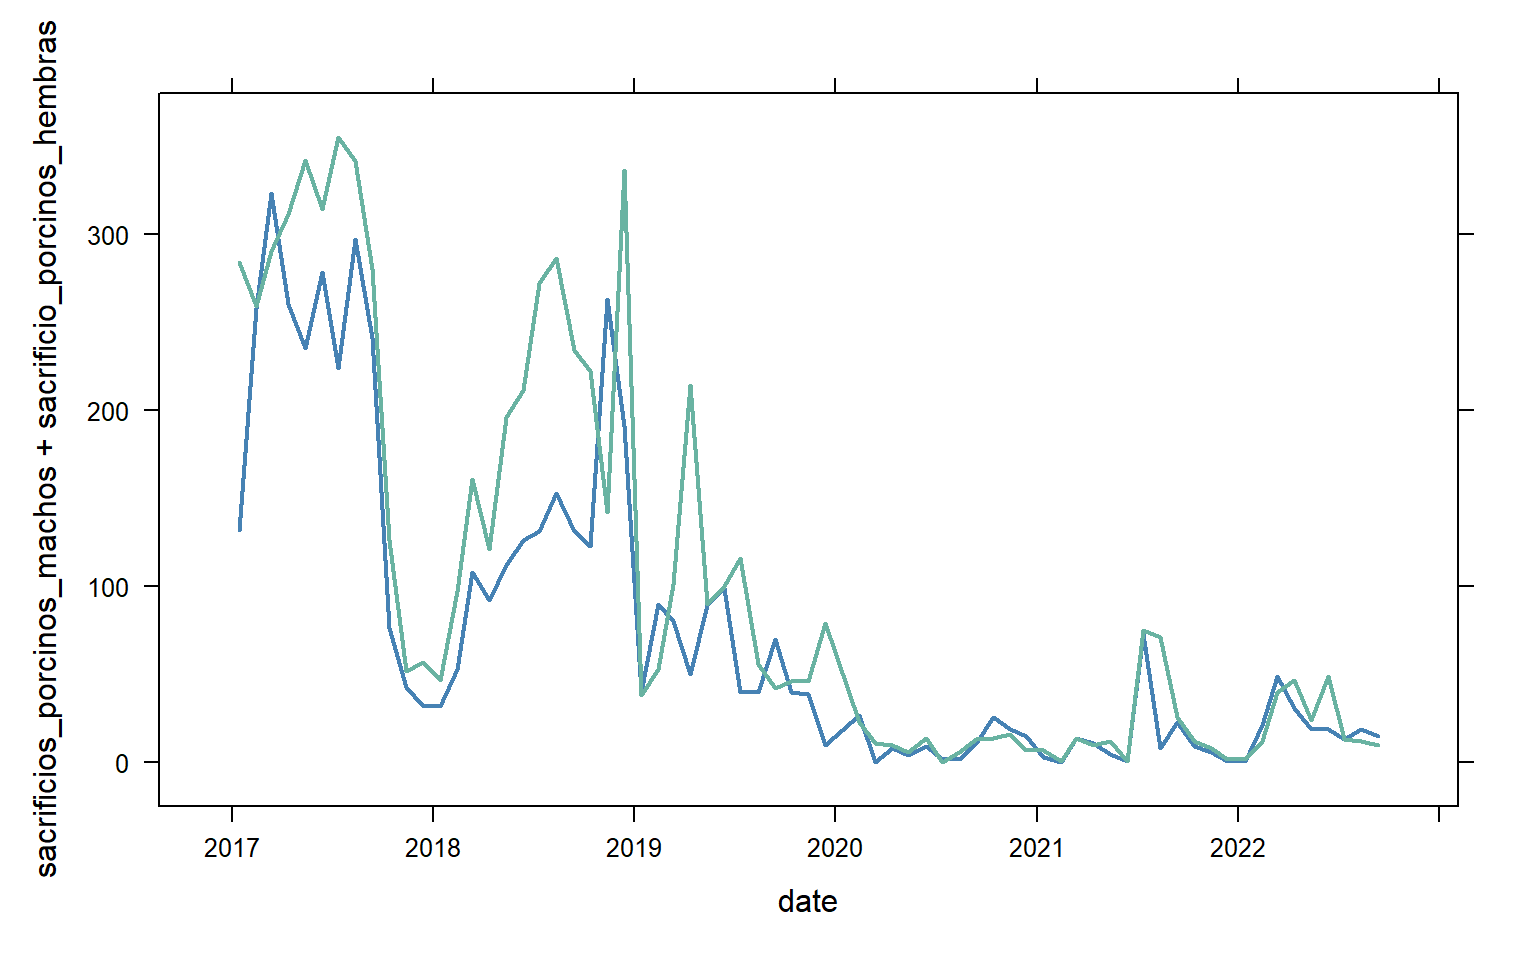
\includegraphics{Tarea-1_Modulo2_files/figure-latex/unnamed-chunk-7-1.pdf}

A continuación se observa un resumen de cada variable.

\begin{Shaded}
\begin{Highlighting}[]
\KeywordTok{summary}\NormalTok{(df)}
\end{Highlighting}
\end{Shaded}

\begin{verbatim}
##       Year          Volume              Today            Direction 
##  Min.   :2015   Min.   :  3014800   Min.   :-1.896e-01   down:581  
##  1st Qu.:2016   1st Qu.:  8348050   1st Qu.:-7.044e-03   up  :670  
##  Median :2017   Median : 11584300   Median : 5.137e-04             
##  Mean   :2017   Mean   : 14584736   Mean   : 8.298e-05             
##  3rd Qu.:2018   3rd Qu.: 17007000   3rd Qu.: 8.902e-03             
##  Max.   :2019   Max.   :138698900   Max.   : 1.219e-01             
##       lag1                 lag2                 lag3           
##  Min.   :-1.896e-01   Min.   :-0.1896439   Min.   :-0.1896439  
##  1st Qu.:-7.044e-03   1st Qu.:-0.0070049   1st Qu.:-0.0070049  
##  Median : 5.137e-04   Median : 0.0005164   Median : 0.0005164  
##  Mean   : 8.435e-05   Mean   : 0.0001094   Mean   : 0.0001149  
##  3rd Qu.: 8.902e-03   3rd Qu.: 0.0089639   3rd Qu.: 0.0089947  
##  Max.   : 1.219e-01   Max.   : 0.1218519   Max.   : 0.1218519  
##       lag4                 lag5           
##  Min.   :-0.1896439   Min.   :-1.896e-01  
##  1st Qu.:-0.0070436   1st Qu.:-7.111e-03  
##  Median : 0.0005137   Median : 5.137e-04  
##  Mean   : 0.0001076   Mean   : 9.421e-05  
##  3rd Qu.: 0.0089947   3rd Qu.: 8.995e-03  
##  Max.   : 0.1218519   Max.   : 1.219e-01
\end{verbatim}

\textbf{b.} Utilizando validación cruzada, encuentre el K (el número de
vecinos), del modelo KNN, que mejores resultados arroje en términos del
error de prueba estimado para predecir si el precio de la acción sube (o
se mantiene igual) o baja en función de los 5 ``lags'' pasados y el
volumen.

Primero dividimos la base de datos en entrenamiento y prueba. Por ser
datos temporales se prefiere tomar como datos de prueba aquellos del año
2019 y el restante como datos de entrenamiento.

\begin{Shaded}
\begin{Highlighting}[]
\NormalTok{train <-}\StringTok{ }\NormalTok{(df}\OperatorTok{$}\NormalTok{Year}\OperatorTok{<}\DecValTok{2019}\NormalTok{)}
\NormalTok{test <-}\StringTok{ }\NormalTok{df[}\OperatorTok{!}\NormalTok{train,] }\CommentTok{# Datos de test}
\NormalTok{train <-}\StringTok{ }\NormalTok{df[train,] }\CommentTok{# Datos de train}
\end{Highlighting}
\end{Shaded}

Luego normalizamos la variable Volumen de la siguiente manera:

\[
z=\frac{x-\min (x)}{\max (x)-\min (x)}
\]

\begin{Shaded}
\begin{Highlighting}[]
\NormalTok{train}\OperatorTok{$}\NormalTok{Volume <-}\StringTok{ }\KeywordTok{normalize}\NormalTok{(train}\OperatorTok{$}\NormalTok{Volume)}
\NormalTok{test}\OperatorTok{$}\NormalTok{Volume <-}\StringTok{ }\KeywordTok{normalize}\NormalTok{(test}\OperatorTok{$}\NormalTok{Volume)}
\NormalTok{y_train <-}\StringTok{ }\NormalTok{train[}\StringTok{"Direction"}\NormalTok{]}
\NormalTok{y_test <-}\StringTok{ }\NormalTok{test[}\StringTok{"Direction"}\NormalTok{]}
\end{Highlighting}
\end{Shaded}

Con ayuda de la librería caret, se usa el método cv (Validación Cruzada)
para indicar que se va a partir la base de entrenamiento en 5 partes
iguales de forma aleatoria (5 fold en inglés). Luego, con su función
trainControl se especifican una serie de parámetros en el modelo. El
objeto que sale de trainControl se proporcionará como argumento para la
función train que se usa para entrenar, de la siguiente manera:

\begin{Shaded}
\begin{Highlighting}[]
\KeywordTok{set.seed}\NormalTok{(}\DecValTok{1233}\NormalTok{)}
\NormalTok{SP_ctrl <-}\StringTok{ }\KeywordTok{trainControl}\NormalTok{(}\DataTypeTok{method=}\StringTok{"cv"}\NormalTok{, }\DataTypeTok{number =} \DecValTok{5}\NormalTok{) }\CommentTok{#5 fold}
\NormalTok{SP_knnEntrenado <-}\StringTok{ }\KeywordTok{train}\NormalTok{(Direction }\OperatorTok{~}\StringTok{ }\NormalTok{., }\DataTypeTok{data =}\NormalTok{ train, }
                \DataTypeTok{method =} \StringTok{"knn"}\NormalTok{, }\DataTypeTok{tuneLength =} \DecValTok{20}\NormalTok{, }\CommentTok{#numeros de k}
                \DataTypeTok{trControl =}\NormalTok{ SP_ctrl,}
                \DataTypeTok{preProcess =} \KeywordTok{c}\NormalTok{(}\StringTok{"center"}\NormalTok{,}\StringTok{"scale"}\NormalTok{))}
\NormalTok{SP_knnEntrenado}
\end{Highlighting}
\end{Shaded}

\begin{verbatim}
## k-Nearest Neighbors 
## 
## 1000 samples
##    8 predictor
##    2 classes: 'down', 'up' 
## 
## Pre-processing: centered (8), scaled (8) 
## Resampling: Cross-Validated (5 fold) 
## Summary of sample sizes: 800, 800, 800, 800, 800 
## Resampling results across tuning parameters:
## 
##   k   Accuracy  Kappa    
##    5  0.854     0.7069691
##    7  0.858     0.7143302
##    9  0.860     0.7184333
##   11  0.866     0.7303060
##   13  0.863     0.7241337
##   15  0.874     0.7460857
##   17  0.881     0.7604922
##   19  0.885     0.7684072
##   21  0.883     0.7641887
##   23  0.884     0.7662885
##   25  0.885     0.7682148
##   27  0.879     0.7560685
##   29  0.879     0.7559757
##   31  0.879     0.7559025
##   33  0.881     0.7598491
##   35  0.881     0.7600719
##   37  0.876     0.7494777
##   39  0.872     0.7413568
##   41  0.876     0.7495291
##   43  0.874     0.7454145
## 
## Accuracy was used to select the optimal model using the largest value.
## The final value used for the model was k = 25.
\end{verbatim}

Así entonces, la presición del modelo resulta ser óptima asignando el
valor de k = 25, como se puede observar en la siguiente gráfica:

\begin{Shaded}
\begin{Highlighting}[]
\KeywordTok{plot}\NormalTok{(SP_knnEntrenado)}
\end{Highlighting}
\end{Shaded}

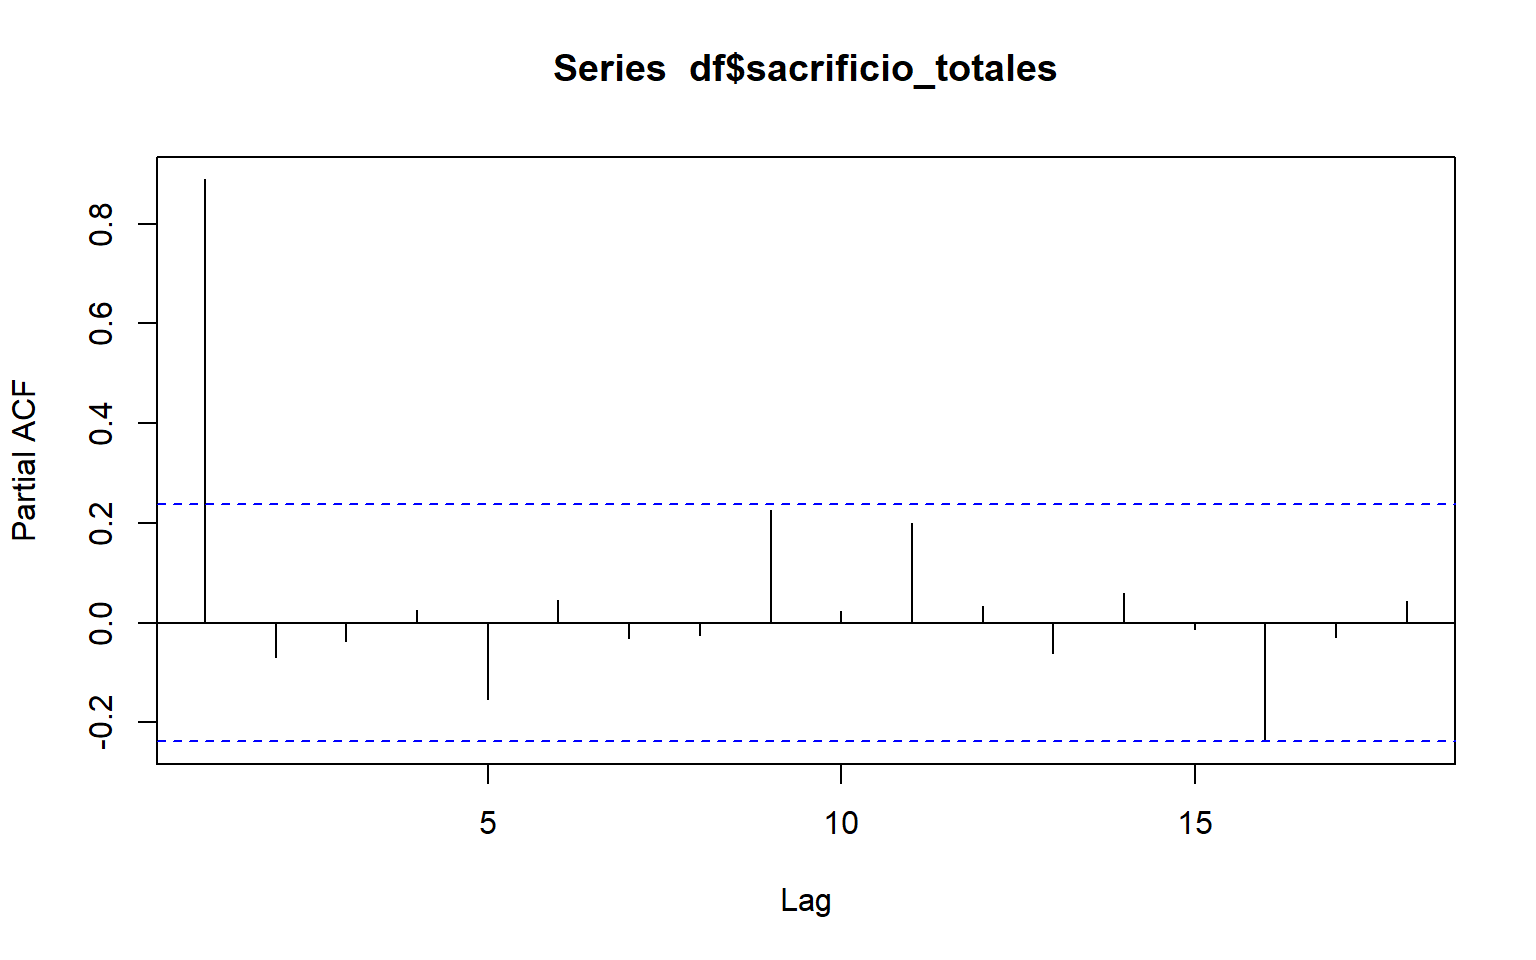
\includegraphics{Tarea-1_Modulo2_files/figure-latex/unnamed-chunk-12-1.pdf}

\textbf{c.} Con los datos de entrenamiento, ajuste un modelo logístico,
un KNN con K encontrado en el item (b), un LDA y un QDA para predecir si
el precio de la acción sube (o se mantiene igual) o baja en función de
los 5 ``lags'' pasados y el volumen. Para cada modelo obtenga la matriz
de confusión y el estimador del error de prueba. Cuál modelo arroja
mejores resultados y por qué?

\textbf{Modelo logístico}

Haciendo uso de la partición de datos del numeral ``b'' ajustamos el
siguiente modelo lógistico, con ``Direction'' como variable
independiente, así entonces, volumen y los cinco rezagos como variables
predictoras:

\begin{Shaded}
\begin{Highlighting}[]
\NormalTok{train <-}\StringTok{ }\NormalTok{(df}\OperatorTok{$}\NormalTok{Year}\OperatorTok{<}\DecValTok{2019}\NormalTok{)}
\NormalTok{test <-}\StringTok{ }\NormalTok{df[}\OperatorTok{!}\NormalTok{train,] }\CommentTok{# Datos de test}
\NormalTok{train <-}\StringTok{ }\NormalTok{df[train,] }\CommentTok{# Datos de train}
\end{Highlighting}
\end{Shaded}

\begin{Shaded}
\begin{Highlighting}[]
\NormalTok{mod_glm <-}\StringTok{ }\KeywordTok{glm}\NormalTok{(Direction }\OperatorTok{~}\StringTok{ }\NormalTok{lag1}\OperatorTok{+}\NormalTok{lag2}\OperatorTok{+}\NormalTok{lag3}\OperatorTok{+}\NormalTok{lag4}\OperatorTok{+}\NormalTok{lag5}\OperatorTok{+}\NormalTok{Volume, }
               \DataTypeTok{data =}\NormalTok{ df[df}\OperatorTok{$}\NormalTok{Year}\OperatorTok{<}\DecValTok{2019}\NormalTok{,], }\DataTypeTok{family =}\NormalTok{ binomial)}
\end{Highlighting}
\end{Shaded}

\begin{Shaded}
\begin{Highlighting}[]
\CommentTok{#matriz de confusión}
\NormalTok{glm.pred <-}\StringTok{ }\KeywordTok{predict}\NormalTok{(mod_glm, test[,}\OperatorTok{-}\DecValTok{4}\NormalTok{], }\DataTypeTok{type=}\StringTok{"response"}\NormalTok{)}
\NormalTok{glm.pred <-}\StringTok{ }\KeywordTok{ifelse}\NormalTok{(glm.pred }\OperatorTok{<}\StringTok{ }\FloatTok{0.53}\NormalTok{, }\StringTok{"down"}\NormalTok{, }\StringTok{"up"}\NormalTok{)}
\NormalTok{t<-}\KeywordTok{table}\NormalTok{(glm.pred, test}\OperatorTok{$}\NormalTok{Direction);t}
\end{Highlighting}
\end{Shaded}

\begin{verbatim}
##         
## glm.pred down  up
##     down   37  40
##     up     74 100
\end{verbatim}

\begin{Shaded}
\begin{Highlighting}[]
\CommentTok{#tasa de acierto}
\KeywordTok{sum}\NormalTok{(}\KeywordTok{diag}\NormalTok{(t))}\OperatorTok{/}\KeywordTok{sum}\NormalTok{ (t)}
\end{Highlighting}
\end{Shaded}

\begin{verbatim}
## [1] 0.5458167
\end{verbatim}

\begin{Shaded}
\begin{Highlighting}[]
\CommentTok{#tasa de error}
\KeywordTok{mean}\NormalTok{(glm.pred}\OperatorTok{!=}\NormalTok{test}\OperatorTok{$}\NormalTok{Direction)}
\end{Highlighting}
\end{Shaded}

\begin{verbatim}
## [1] 0.4541833
\end{verbatim}

Así entonces, la proporción de veces que el modelo logístico predijo
correctamente (accuracy) es de del 54.6\%. Hay que tener en cuenta que
se pueden mejorar estos resultados realizando otro tipo de análisis y
limpieza de los datos.

\textbf{Modelo K-Vecinos más cercanos}

Haciendo uso de la partición de datos del numeral ``b'' ajustamos el
siguiente modelo KNN, con ``Direction'' como variable independiente, así
entonces, volumen y los cinco rezagos como variables predictoras:

\begin{Shaded}
\begin{Highlighting}[]
\NormalTok{train}\OperatorTok{$}\NormalTok{Volume <-}\StringTok{ }\KeywordTok{normalize}\NormalTok{(train}\OperatorTok{$}\NormalTok{Volume)}
\NormalTok{test}\OperatorTok{$}\NormalTok{Volume <-}\StringTok{ }\KeywordTok{normalize}\NormalTok{(test}\OperatorTok{$}\NormalTok{Volume)}
\NormalTok{y_train <-}\StringTok{ }\NormalTok{train[}\StringTok{"Direction"}\NormalTok{]}
\NormalTok{y_test <-}\StringTok{ }\NormalTok{test[}\StringTok{"Direction"}\NormalTok{]}
\end{Highlighting}
\end{Shaded}

\begin{Shaded}
\begin{Highlighting}[]
\KeywordTok{set.seed}\NormalTok{(}\DecValTok{1233}\NormalTok{)}
\NormalTok{fit.knn_train <-}\StringTok{ }\NormalTok{class}\OperatorTok{::}\KeywordTok{knn}\NormalTok{(}\DataTypeTok{train=}\NormalTok{train[,}\OperatorTok{-}\DecValTok{4}\NormalTok{], }\DataTypeTok{test=}\NormalTok{ train[,}\OperatorTok{-}\DecValTok{4}\NormalTok{], }
                            \DataTypeTok{cl =}\NormalTok{ y_train}\OperatorTok{$}\NormalTok{Direction, }\DataTypeTok{k=}\DecValTok{25}\NormalTok{, }\DataTypeTok{prob=}\OtherTok{TRUE}\NormalTok{)}
\end{Highlighting}
\end{Shaded}

\begin{Shaded}
\begin{Highlighting}[]
\NormalTok{fit.knn_Test <-}\StringTok{ }\NormalTok{class}\OperatorTok{::}\KeywordTok{knn}\NormalTok{(}\DataTypeTok{train=}\NormalTok{train[,}\OperatorTok{-}\DecValTok{4}\NormalTok{], }\DataTypeTok{test =}\NormalTok{ test[,}\OperatorTok{-}\DecValTok{4}\NormalTok{], }
                         \DataTypeTok{cl=}\NormalTok{ y_train}\OperatorTok{$}\NormalTok{Direction, }\DataTypeTok{k=}\DecValTok{25}\NormalTok{, }\DataTypeTok{prob=}\OtherTok{TRUE}\NormalTok{)}
\end{Highlighting}
\end{Shaded}

\begin{Shaded}
\begin{Highlighting}[]
\CommentTok{#matriz de confusión}
\NormalTok{Predicted_test<-}\KeywordTok{factor}\NormalTok{(fit.knn_Test)}
\NormalTok{t1<-}\KeywordTok{table}\NormalTok{(Predicted_test,y_test}\OperatorTok{$}\NormalTok{Direction)}
\NormalTok{t1}
\end{Highlighting}
\end{Shaded}

\begin{verbatim}
##               
## Predicted_test down  up
##           down   86  26
##           up     25 114
\end{verbatim}

\begin{Shaded}
\begin{Highlighting}[]
\CommentTok{#tasa de acierto}
\KeywordTok{sum}\NormalTok{(}\KeywordTok{diag}\NormalTok{(t1))}\OperatorTok{/}\KeywordTok{sum}\NormalTok{(t1)}
\end{Highlighting}
\end{Shaded}

\begin{verbatim}
## [1] 0.7968127
\end{verbatim}

\begin{Shaded}
\begin{Highlighting}[]
\CommentTok{#tasa de error}
\KeywordTok{mean}\NormalTok{(Predicted_test}\OperatorTok{!=}\NormalTok{test}\OperatorTok{$}\NormalTok{Direction)}
\end{Highlighting}
\end{Shaded}

\begin{verbatim}
## [1] 0.2031873
\end{verbatim}

Así entonces, la proporción de veces que el modelo KNN predijo
correctamente (accuracy) es de 79.7\%. Hay que tener en cuenta que se
pueden mejorar estos resultados realizando otro tipo de análisis y
limpieza de los datos.

\textbf{Modelo Análisis de discriminante linea LDA}

Es una alternativa a la regresión logística cuando la variable
cualitativa tiene más de dos niveles. Si bien existen extensiones de la
regresión logística para múltiples clases, el LDA presenta una serie de
ventajas

Haciendo uso de la partición de datos del numeral ``b'' ajustamos el
siguiente modelo LDA, con ``Direction'' como variable independiente, así
entonces, volumen y los cinco rezagos como variables predictoras:

\begin{Shaded}
\begin{Highlighting}[]
\NormalTok{train <-}\StringTok{ }\NormalTok{(df}\OperatorTok{$}\NormalTok{Year}\OperatorTok{<}\DecValTok{2019}\NormalTok{)}
\NormalTok{test <-}\StringTok{ }\NormalTok{df[}\OperatorTok{!}\NormalTok{train,] }\CommentTok{# Datos de test}
\NormalTok{train <-}\StringTok{ }\NormalTok{df[train,] }\CommentTok{# Datos de train}
\end{Highlighting}
\end{Shaded}

\begin{Shaded}
\begin{Highlighting}[]
\NormalTok{mod_lda <-}\StringTok{ }\NormalTok{MASS}\OperatorTok{::}\KeywordTok{lda}\NormalTok{(Direction}\OperatorTok{~}\NormalTok{lag1}\OperatorTok{+}\NormalTok{lag2}\OperatorTok{+}\NormalTok{lag3}\OperatorTok{+}\NormalTok{lag4}\OperatorTok{+}\NormalTok{lag5}\OperatorTok{+}\NormalTok{Volume,}\DataTypeTok{data =}\NormalTok{ train)}
\NormalTok{mod_lda}
\end{Highlighting}
\end{Shaded}

\begin{verbatim}
## Call:
## lda(Direction ~ lag1 + lag2 + lag3 + lag4 + lag5 + Volume, data = train)
## 
## Prior probabilities of groups:
## down   up 
## 0.47 0.53 
## 
## Group means:
##               lag1          lag2          lag3          lag4          lag5
## down -0.0003185799 -0.0003620329 -2.434966e-05 -0.0009251057  0.0003099079
## up    0.0004640592  0.0005508848  2.687681e-04  0.0009628981 -0.0001378771
##        Volume
## down 16047804
## up   14755668
## 
## Coefficients of linear discriminants:
##                  LD1
## lag1    1.258587e+01
## lag2    1.441198e+01
## lag3    3.739337e+00
## lag4    3.138705e+01
## lag5   -1.186942e+01
## Volume -5.869769e-08
\end{verbatim}

La salida LDA indica que el 47\% de las observaciones de entrenamiento
corresponden a días en los que el mercado bajó. Los coeficientes de
salida de los discriminantes lineales proporcionan la combinación lineal
del volumen y los rezagos que se utilizan para formar la regla de
decisión LDA.

\begin{Shaded}
\begin{Highlighting}[]
\CommentTok{#matriz de confusión}
\NormalTok{Pred.lda<-}\KeywordTok{predict}\NormalTok{(mod_lda , test) }
\NormalTok{Clase.lda =}\StringTok{ }\NormalTok{Pred.lda}\OperatorTok{$}\NormalTok{class }
\NormalTok{t<-}\KeywordTok{table}\NormalTok{(Clase.lda,test}\OperatorTok{$}\NormalTok{Direction);t}
\end{Highlighting}
\end{Shaded}

\begin{verbatim}
##          
## Clase.lda down  up
##      down   11  12
##      up    100 128
\end{verbatim}

\begin{Shaded}
\begin{Highlighting}[]
\CommentTok{#tasa de acierto}
\KeywordTok{sum}\NormalTok{(}\KeywordTok{diag}\NormalTok{(t))}\OperatorTok{/}\KeywordTok{sum}\NormalTok{(t)}
\end{Highlighting}
\end{Shaded}

\begin{verbatim}
## [1] 0.5537849
\end{verbatim}

\begin{Shaded}
\begin{Highlighting}[]
\CommentTok{#tasa de error}
\KeywordTok{mean}\NormalTok{(Clase.lda}\OperatorTok{!=}\NormalTok{test}\OperatorTok{$}\NormalTok{Direction)}
\end{Highlighting}
\end{Shaded}

\begin{verbatim}
## [1] 0.4462151
\end{verbatim}

Así entonces, la proporción de veces que el modelo LDA predijo
correctamente (accuracy) es de 55.4\%. Hay que tener en cuenta que se
pueden mejorar estos resultados realizando otro tipo de análisis y
limpieza de los datos.

\textbf{Modelo QDA (Análisis discriminante cuadrático)}

Haciendo uso de la partición de datos del numeral ``b'' ajustamos el
siguiente modelo QDA, con ``Direction'' como variable independiente, así
entonces, volumen y los cinco rezagos como variables predictoras:

\begin{Shaded}
\begin{Highlighting}[]
\NormalTok{mod_qda <-}\StringTok{ }\NormalTok{MASS}\OperatorTok{::}\KeywordTok{qda}\NormalTok{(Direction}\OperatorTok{~}\NormalTok{lag1}\OperatorTok{+}\NormalTok{lag2}\OperatorTok{+}\NormalTok{lag3}\OperatorTok{+}\NormalTok{lag4}\OperatorTok{+}\NormalTok{lag5}\OperatorTok{+}\NormalTok{Volume, }\DataTypeTok{data =}\NormalTok{ train)}
\NormalTok{mod_qda}
\end{Highlighting}
\end{Shaded}

\begin{verbatim}
## Call:
## qda(Direction ~ lag1 + lag2 + lag3 + lag4 + lag5 + Volume, data = train)
## 
## Prior probabilities of groups:
## down   up 
## 0.47 0.53 
## 
## Group means:
##               lag1          lag2          lag3          lag4          lag5
## down -0.0003185799 -0.0003620329 -2.434966e-05 -0.0009251057  0.0003099079
## up    0.0004640592  0.0005508848  2.687681e-04  0.0009628981 -0.0001378771
##        Volume
## down 16047804
## up   14755668
\end{verbatim}

\begin{Shaded}
\begin{Highlighting}[]
\CommentTok{#matriz de confusion}
\NormalTok{Pred.qda<-}\KeywordTok{predict}\NormalTok{(mod_qda , test) }
\NormalTok{Clase.qda =Pred.qda}\OperatorTok{$}\NormalTok{class}
\NormalTok{t1<-}\KeywordTok{table}\NormalTok{(Clase.qda, test}\OperatorTok{$}\NormalTok{Direction);t1}
\end{Highlighting}
\end{Shaded}

\begin{verbatim}
##          
## Clase.qda down  up
##      down   13  13
##      up     98 127
\end{verbatim}

\begin{Shaded}
\begin{Highlighting}[]
\CommentTok{#Tasa de acierto}
\KeywordTok{sum}\NormalTok{(}\KeywordTok{diag}\NormalTok{(t1))}\OperatorTok{/}\KeywordTok{sum}\NormalTok{(t1) }
\end{Highlighting}
\end{Shaded}

\begin{verbatim}
## [1] 0.5577689
\end{verbatim}

Así entonces, la proporción de veces que el modelo QDA predijo
correctamente (accuracy) es del 55.8\%. Hay que tener en cuenta que se
pueden mejorar estos resultados realizando otro tipo de análisis y
limpieza de los datos.

\textbf{Cuál modelo arroja mejores resultados y por qué?}

\begin{itemize}
\tightlist
\item
  Los modelos logístico, QDA y LDA obtuvieron una tasa de aciertos
  similar 54.6\%, 55.4\% y 55.8\% respectivamente. La exactitud
  (accuracy) más alto fue de 79.7\% obtenido por el modelo KNN, teniendo
  en cuenta que este último es más flexible y tuvo la ventaja con
  respecto a los otros modelos de utilizar validación cruzada para
  minimizar su error.
\end{itemize}

\textbf{2. Resuelva el ejercicio 3 de la sección 4.7 del texto}

Este problema se relaciona con el modelo QDA, en el que las
observaciones dentro de cada clase se extraen de una distribución normal
con un vector medio específico de la clase y una matriz de covarianza
específica de la clase. Consideramos el caso simple donde p = 1; es
decir, solo hay una característica.

Suponga que tenemos K clases, y que si una observación pertenece a la
k-ésima clase, entonces X proviene de una distribución normal
unidimensional, X \(\sim\) N ( \(\mu_k\), \(\sigma_k^2\)). Recuerde que
la función de densidad para la distribución normal unidimensional se da
en (4.11). Demuestre que en este caso, el clasificador de Bayes no es
lineal. Argumenta que de hecho es cuadrático.

Sugerencia: Para este problema, debe seguir los argumentos establecidos
en la Sección 4.4.2, pero sin asumir que \(\sigma_1^2\) =. . . =
\(\sigma_K^2\).

\[
p_k(x) = \frac {\pi_k
                \frac {1} {\sqrt{2 \pi} \sigma_k}
                \exp(- \frac {1} {2 \sigma_k^2} (x - \mu_k)^2)
               }
               {\sum_{l = 1}^K{
                \pi_l
                \frac {1} {\sqrt{2 \pi} \sigma_l}
                \exp(- \frac {1} {2 \sigma_l^2} (x - \mu_l)^2)
               }}
\] \[
\log(p_k(x)) = \frac {\log(\pi_k) +
                \log(\frac {1} {\sqrt{2 \pi} \sigma_k}) + 
                - \frac {1} {2 \sigma_k^2} (x - \mu_k)^2
               }
               {\log(\sum_{l = 1}^K {
                \pi_l
                \frac {1} {\sqrt{2 \pi} \sigma_l}
                \exp(- \frac {1} {2 \sigma_l^2} (x - \mu_l)^2)
               })}
\]

\[
\log(p_k(x)) = \log(\pi_k) +
                \log(\frac {1} {\sqrt{2 \pi} \sigma_k}) 
                - \frac {1} {2 \sigma_k^2} (x - \mu_k)^2
                -
               \log(\sum_{l = 1}^K {
                \pi_l
                \frac {1} {\sqrt{2 \pi} \sigma_l}
                \exp(- \frac {1} {2 \sigma_l^2} (x - \mu_l)^2)
               })
\]

Como el último termino
\(\log(\sum_{l = 1}^K {  \pi_l  \frac {1} {\sqrt{2 \pi} \sigma_l}  \exp(- \frac {1} {2 \sigma_l^2} (x - \mu_l)^2)  })\),
es independiente de k, este será un termino constante \(\forall\) k pues
es una sumatoria sobre K(grande), por lo cual, queda hallar k en el cual
se maximiza:

\[
\log(\pi_k) +
  \log(\frac {1} {\sqrt{2 \pi} \sigma_k})  
  - \frac {1} {2 \sigma_k^2} (x - \mu_k)^2
\]

\[
= log(\pi_k) + log(\frac{1}{\sqrt{2\pi}\sigma_k}) -  \frac{x^2}{2\sigma_k^2} + x \cdot \frac{\mu_k}{\sigma_k^2}  - \frac{\mu_k^2}{2\sigma_k} 
\]

Con lo anterior: \[
\delta_k(x)
= log(\pi_k) + log(\frac{1}{\sqrt{2\pi}\sigma_k}) -  \frac{x^2}{2\sigma_k^2} + x \cdot \frac{\mu_k}{\sigma_k^2}  - \frac{\mu_k^2}{2\sigma_k} 
\]

Como se observa, \(\delta_k(x)\) no es una ecuación lineal pues depende
de un termino cuadrático en x.

\textbf{3.}Pruebe que si en el modelo de regresión lineal múltiple se
tiene que \(p > n\) (el número de covariables es mayor que el tamaño
muestral) entonces los estimadores de los
coeficientes,\(\widehat{\beta }\) , no son únicos. ¿Cuáles son las
alternativas para ``resolver'' este problema?

Para la regresión lineal múltiple, los coeficientes de regresión se
pueden estimar por mínimos cuadrados, Suponiendo lo contrario que se
plantea en el punto y que \$n \textgreater{} p \$, se tiene a \(y_{i}\)
la cual es la i-ésima respuesta observada y \(x_{ij}\) la i-ésima
observación; también se supone que el término del error \(\varepsilon\)
tiene \(E\left ( \varepsilon \right ) = 0\) y
\(Var\left ( \varepsilon \right ) = \sigma ^{2}\), y los errores no
estan correlacionados.

El modelo muestral de regresión se puede escribir como:

\[
y_{i}=\beta _{0}+\beta _{1}x_{i1}+\beta _{1}x_{i2}+\ ...\ +\beta _{k}x_{ik} +\varepsilon _{i}\\
y_{i}=\beta _{0}+\sum_{j=1}^{k}\beta _{j}x_{ij} +\ \varepsilon _{i},  \ i=1,2,...n
\] La función de mínimos cuadrados es

\[
S\left ( \beta _{0},\beta _{1}, ..., \beta _{k} \right ) = \sum_{i = 1}^{n}\varepsilon _{i}^{2}\\
 = \sum_{i = 1}^{n}\left ( y_{i}-\beta _{0}-\sum_{j=1}^{k}\beta _{j}x_{ij} \right )^{2}
\] Se debe minimizar la función \(S\) respecto a
\(\beta _{0},\beta _{1}, ..., \beta _{k}\). Los estimadores de
\(\beta _{0},\beta _{1}, ..., \beta _{k}\) por mínimos cuadrados deben
satisfacer

\$\$
\frac{\partial S}{\partial \beta _{0}}\mid \emph{\{\widehat{\beta _{0}},\{\widehat\beta }\{2\},\ldots,\widehat\beta \emph{\{k\}\}\}
= -2\sum}\{i=1\}\^{}\{n\}\left (
y\_\{i\}-\widehat{\beta _{0}}-\sum\emph{\{j=1\}\^{}\{k\}\widehat{\beta_{j}}x}\{ij\}
\right ) = 0\textbackslash{}

\frac{\partial S}{\partial \beta _{j}}\mid \emph{\{\widehat{\beta _{0}},\{\widehat\beta }\{2\},\ldots,\widehat\beta \emph{\{k\}\}\}
= -2\sum}\{i=1\}\^{}\{n\}\left (
y\_\{i\}-\widehat{\beta _{0}}-\sum\emph{\{j=1\}\^{}\{k\}\widehat{\beta_{j}}x}\{ij\}
\right )x\_\{ij\} = 0, ~j ~= ~1,2,\ldots,k \$\$ Al simplificar la
ecuación se obtienen las ecuaciones normales de mínimos cuadrados

\$\$ n\widehat{\beta _{0}} +
\widehat{\beta _{1}}\sum\emph{\{i=1\}\^{}\{n\}x}\{i1\} +
\widehat{\beta _{2}}\sum\emph{\{i=1\}\^{}\{n\}x}\{i2\} + \ldots{} +
\widehat{\beta _{k}}\sum\emph{\{i=1\}\^{}\{n\}x}\{ik\} =
\sum\emph{\{i=1\}\^{}\{n\}y}\{i\}\textbackslash{}

\widehat{\beta _{0}}\sum\emph{\{i=1\}\^{}\{n\}x}\{i1\} +
\widehat{\beta _{1}}\sum\emph{\{i=1\}\textsuperscript{\{n\}x\_\{i1\}}\{2\}
+ \widehat{\beta _{2}}\sum}\{i=1\}\^{}\{n\}x\_\{i1\}x\_\{i2\} + \ldots{}
+ \widehat{\beta _{k}}\sum\emph{\{i=1\}\^{}\{n\}x}\{i1\}x\_\{ik\} =
\sum\emph{\{i=1\}\^{}\{n\}x}\{i1\}y\_\{i\}\textbackslash{}

\vdots  \textbackslash{}

\widehat{\beta _{0}}\sum\emph{\{i=1\}\^{}\{n\}x}\{ik\} +
\widehat{\beta _{1}}\sum\emph{\{i=1\}\^{}\{n\}x}\{ik\}x\_\{i1\} +
\widehat{\beta _{2}}\sum\emph{\{i=1\}\^{}\{n\}x}\{ik\}x\_\{i2\} +
\ldots{} +
\widehat{\beta _{k}}\sum\emph{\{i=1\}\textsuperscript{\{n\}x\_\{ik\}}2
=\sum}\{i=1\}\^{}\{n\}x\_\{ik\}y\_\{i\}\textbackslash{} \$\$

Se sae que \(p = k + 1\), se mostratra de forma matricial

\[
y =X\beta + \varepsilon 
\]

Se determina el estimador de \(\widehat{\beta}\) por minimos cuadrados:

\$\$ S(\beta )= \sum\emph{\{i=1\}\^{}\{n\}\varepsilon }\{i\}\^{}2 =
\varepsilon {}' ~\varepsilon  = (y -
X\beta )\{\}'(y-X\beta )\textbackslash{}

S(\beta )= y\{\}'y- \beta {X}'y - y\{\}'X\beta +
\beta {}'X\{\}'X\beta \textbackslash{}

S(\beta )= y\{\}'y- 2 \beta {X}'y + \beta {}'X\{\}'X\beta  \[
Los estimadores de mínimos cuadrados deben satisfacer 
\]

X\{\}'X\widehat{\beta }=X\{\}'y\textbackslash{} \widehat{\beta }=\left (
X\{\}'X\right )\^{}\{-1\}X\{\}'y \$\$ Como se logra ver ese seria el
estimador de los \(\widehat{\beta}\) y se supone que la matriz inversa
\$ \left ( X\{\}'X\right )\^{}\{-1\}\$ siempre existe si los regresores
son linealmente independientes.

Es decir, la estimación está bien definida cuando las variables
predictoras, es decir, las columnas de x, son linealmente
independientes. Pero cuando \(p> n\), la matriz \(X\) no puede tener
columnas linealmente independientes, \$ y \(X^{T}X\) es no invertible,
pues como hay mas covariables hay la posibilidad de multicolinealidad,
también al tener un tamaño de muestra pequeño la regresión lineal
múltiple se ajusta a los pocos puntos , dando un problema de ajuste,para
poder dar predicción , por esto si el modelo, se utiliza para dar
predicciones o se cambia la base de datos, los \(\widehat{\beta}\)
cambiarian completamente, y no tendrian un rango de estimación, además
que su \(R^{2}\) podria ser muy cercano a 1 , pero seria una mala
estimación.

Hay varias maneras de arreglar las cuales serian:

\begin{itemize}
\tightlist
\item
  Selección de subconjuntos de covariables: Las covariables más
  relevantes para explicar la variabilidad de Y son seleccionadas, es
  decir, las que expliquen la mayor variabilidad de Y, y no haya
  multicolinealidad.
\end{itemize}

-Reducción de dimensionalidad: Consiste en proyectar las p covariables
en un subespacio de dimensión reducida, \(M\), con \(M < p\). Esto
produce \(M\) combinaciones lineales de las variables originales y
dichas combinaciones se usan luego como predictores o covariables.

\begin{itemize}
\tightlist
\item
  la selección progresiva hacia adelante, la regresión de crestas, el
  lazo y la regresión de componentes principales, son particularmente
  útil para realizar regresiones en entornos de alta dimensión, es decir
  , mayor número de covariables que tamalo de muestra \(p > n\).
  Esencialmente, estos enfoques evitan el sobreajuste mediante el uso de
  un enfoque de ajuste menos flexible que los mínimos cuadrados.
\end{itemize}

Al utilizar estos modelos en entornos de alta dimensión, siempre tener
en centa:

-La regularización o la contracción juega un papel clave en un entorno
de alta dimensión \((p> n)\).

-La selección del parámetro de ajuste apropiado es clave para una buena
precisión de predicción

-El error de prueba aumentará a medida que aumente la dimensionalidad
del problema.

\textbf{4.}

\textbf{a.} Se simula una base de datos considerando el modelo lineal
\(Y=X\beta+\epsilon\), teniendo en cuenta las siguientes condicines:

\begin{itemize}
\tightlist
\item
  \(Y\): es una variable numérica dependiente.
\item
  \(X_1\), \(X_2\) y \(X_3\) son variables numéricas independientes.
\item
  \(X_4\) es una variable categórica independiente con tres categorías.
\item
  \((\beta_0,\beta_1,\beta_2,\beta_3,\beta_4,\beta_5)^T=(1,0.3,0.6,-1,1.5,-2)^T\)
\item
  \(\epsilon \sim T-studen(9)\)
\item
  \(n=500\).
\end{itemize}

\begin{Shaded}
\begin{Highlighting}[]
\KeywordTok{set.seed}\NormalTok{(}\DecValTok{123}\NormalTok{)}
\CommentTok{# Valores para la simulación}
\NormalTok{n <-}\StringTok{ }\DecValTok{500}

\NormalTok{x1 <-}\StringTok{ }\KeywordTok{runif}\NormalTok{(}\DataTypeTok{n =}\NormalTok{ n, }\DataTypeTok{min =} \DecValTok{0}\NormalTok{, }\DataTypeTok{max =} \DecValTok{1}\NormalTok{)}
\NormalTok{x2 <-}\StringTok{ }\KeywordTok{rpois}\NormalTok{(}\DataTypeTok{n =}\NormalTok{ n, }\DataTypeTok{lambda =} \DecValTok{3}\NormalTok{)}
\NormalTok{x3 <-}\StringTok{ }\KeywordTok{rgamma}\NormalTok{(}\DataTypeTok{n =}\NormalTok{ n, }\DataTypeTok{shape =} \DecValTok{3}\NormalTok{, }\DataTypeTok{scale =} \DecValTok{2}\NormalTok{, )}
\NormalTok{x4 <-}\StringTok{ }\KeywordTok{c}\NormalTok{(}\StringTok{'A'}\NormalTok{, }\StringTok{'B'}\NormalTok{, }\StringTok{'C'}\NormalTok{)}
\NormalTok{x4 <-}\StringTok{ }\KeywordTok{sample}\NormalTok{(x4, n, }\DataTypeTok{replace =}\NormalTok{ T)}

\CommentTok{# Matriz X del modelo}
\NormalTok{x <-}\StringTok{ }\KeywordTok{model.matrix}\NormalTok{(}\OperatorTok{~}\StringTok{ }\NormalTok{x1}\OperatorTok{+}\NormalTok{x2}\OperatorTok{+}\NormalTok{x3}\OperatorTok{+}\NormalTok{x4)}

\CommentTok{# Vector verdadero de parámetros}
\NormalTok{beta <-}\StringTok{ }\KeywordTok{c}\NormalTok{(}\DecValTok{1}\NormalTok{, }\FloatTok{0.3}\NormalTok{, }\FloatTok{0.6}\NormalTok{, }\DecValTok{-1}\NormalTok{, }\FloatTok{1.5}\NormalTok{, }\DecValTok{-2}\NormalTok{)}
\NormalTok{error <-}\StringTok{ }\KeywordTok{rt}\NormalTok{(n,}\DecValTok{9}\NormalTok{)}

\CommentTok{# Variable respuesta}
\NormalTok{y <-}\StringTok{ }\NormalTok{x }\OperatorTok\StringTok{ }\NormalTok{beta }\OperatorTok{+}\StringTok{ }\NormalTok{error}

\CommentTok{# Base de datos con la simulación hecha}
\NormalTok{datos <-}\StringTok{ }\KeywordTok{data.frame}\NormalTok{(y, x[,}\DecValTok{2}\OperatorTok{:}\DecValTok{6}\NormalTok{])}
\end{Highlighting}
\end{Shaded}

Ahora, utilizando bootstrap se obtendrán intervalos de confianza al 95\%
para \(\sigma\), \(R^2\) y \(R^2-Ajustado\).

\begin{Shaded}
\begin{Highlighting}[]
\KeywordTok{library}\NormalTok{(boot)}
\end{Highlighting}
\end{Shaded}

\begin{verbatim}
## 
## Attaching package: 'boot'
\end{verbatim}

\begin{verbatim}
## The following object is masked from 'package:survival':
## 
##     aml
\end{verbatim}

\begin{verbatim}
## The following object is masked from 'package:lattice':
## 
##     melanoma
\end{verbatim}

\begin{Shaded}
\begin{Highlighting}[]
\CommentTok{#IC para sigma }
\NormalTok{sigma <-}\StringTok{ }\ControlFlowTok{function}\NormalTok{(datos,i)\{}
\NormalTok{  mod =}\StringTok{ }\KeywordTok{lm}\NormalTok{(y}\OperatorTok{~}\NormalTok{x, }\DataTypeTok{data =}\NormalTok{ datos, }\DataTypeTok{subset =}\NormalTok{ i)}
  \KeywordTok{summary}\NormalTok{(mod)}\OperatorTok{$}\NormalTok{sigma}
\NormalTok{\}}

\NormalTok{boot1 <-}\StringTok{ }\KeywordTok{boot}\NormalTok{(datos,sigma,}\DataTypeTok{R=}\DecValTok{500}\NormalTok{)}

\KeywordTok{boot.ci}\NormalTok{(boot1,}\DataTypeTok{conf =} \FloatTok{0.95}\NormalTok{,}\DataTypeTok{type =} \StringTok{"all"}\NormalTok{)}
\end{Highlighting}
\end{Shaded}

\begin{verbatim}
## BOOTSTRAP CONFIDENCE INTERVAL CALCULATIONS
## Based on 500 bootstrap replicates
## 
## CALL : 
## boot.ci(boot.out = boot1, conf = 0.95, type = "all")
## 
## Intervals : 
## Level      Normal              Basic         
## 95%   ( 1.007,  1.165 )   ( 1.005,  1.165 )  
## 
## Level     Percentile            BCa          
## 95%   ( 0.983,  1.144 )   ( 1.007,  1.173 )  
## Calculations and Intervals on Original Scale
## Some BCa intervals may be unstable
\end{verbatim}

\begin{Shaded}
\begin{Highlighting}[]
\CommentTok{#IC para R2}
\NormalTok{r2 <-}\StringTok{ }\ControlFlowTok{function}\NormalTok{ (datos,i)\{}
\NormalTok{  mod =}\StringTok{ }\KeywordTok{lm}\NormalTok{(y}\OperatorTok{~}\NormalTok{x , }\DataTypeTok{data =}\NormalTok{ datos, }\DataTypeTok{subset =}\NormalTok{ i)}
  \KeywordTok{summary}\NormalTok{(mod)}\OperatorTok{$}\NormalTok{r.squared}
\NormalTok{\}}

\NormalTok{boot2 <-}\StringTok{ }\KeywordTok{boot}\NormalTok{(datos,r2,}\DataTypeTok{R=}\DecValTok{500}\NormalTok{)}

\KeywordTok{boot.ci}\NormalTok{(boot2,}\DataTypeTok{conf =} \FloatTok{0.95}\NormalTok{,}\DataTypeTok{type =} \StringTok{"all"}\NormalTok{)}
\end{Highlighting}
\end{Shaded}

\begin{verbatim}
## BOOTSTRAP CONFIDENCE INTERVAL CALCULATIONS
## Based on 500 bootstrap replicates
## 
## CALL : 
## boot.ci(boot.out = boot2, conf = 0.95, type = "all")
## 
## Intervals : 
## Level      Normal              Basic         
## 95%   ( 0.9084,  0.9419 )   ( 0.9099,  0.9442 )  
## 
## Level     Percentile            BCa          
## 95%   ( 0.9053,  0.9396 )   ( 0.9050,  0.9395 )  
## Calculations and Intervals on Original Scale
\end{verbatim}

\begin{Shaded}
\begin{Highlighting}[]
\CommentTok{#IC para R2 ajustado}
\NormalTok{r2adj <-}\StringTok{ }\ControlFlowTok{function}\NormalTok{ (datos,i)\{}
\NormalTok{  mod =}\StringTok{ }\KeywordTok{lm}\NormalTok{(y}\OperatorTok{~}\NormalTok{x , }\DataTypeTok{data =}\NormalTok{ datos, }\DataTypeTok{subset =}\NormalTok{ i)}
  \KeywordTok{summary}\NormalTok{(mod)}\OperatorTok{$}\NormalTok{adj.r.squared}
\NormalTok{\}}

\NormalTok{boot3 <-}\StringTok{ }\KeywordTok{boot}\NormalTok{(datos,r2adj,}\DataTypeTok{R=}\DecValTok{500}\NormalTok{)}

\KeywordTok{boot.ci}\NormalTok{(boot3,}\DataTypeTok{conf =} \FloatTok{0.95}\NormalTok{, }\DataTypeTok{type =} \StringTok{"all"}\NormalTok{)}
\end{Highlighting}
\end{Shaded}

\begin{verbatim}
## BOOTSTRAP CONFIDENCE INTERVAL CALCULATIONS
## Based on 500 bootstrap replicates
## 
## CALL : 
## boot.ci(boot.out = boot3, conf = 0.95, type = "all")
## 
## Intervals : 
## Level      Normal              Basic         
## 95%   ( 0.9076,  0.9392 )   ( 0.9090,  0.9416 )  
## 
## Level     Percentile            BCa          
## 95%   ( 0.9064,  0.9389 )   ( 0.9007,  0.9373 )  
## Calculations and Intervals on Original Scale
## Some BCa intervals may be unstable
\end{verbatim}

Se sabe que los errores siguen una distibucion t-student con 9 grados de
libertad, por lo que su varianza se calcula como v/(v-2), donde v son
los grados de libertad y esto es para v\textgreater2, así, se tiene que
la varianza teórica esperada para los errores es:

\begin{Shaded}
\begin{Highlighting}[]
\NormalTok{v <-}\StringTok{ }\DecValTok{9}   
\NormalTok{var_esp <-}\StringTok{ }\NormalTok{v}\OperatorTok{/}\NormalTok{(v}\DecValTok{-2}\NormalTok{)   }
\NormalTok{var_esp}
\end{Highlighting}
\end{Shaded}

\begin{verbatim}
## [1] 1.285714
\end{verbatim}

\textbf{b.} Simulando de nuevo el modelo del literal anterior pero ahora
incluyendo un término cúbico para \(X_1\) con coeficiente
\(\beta_{13}=2\), se tiene:

\begin{Shaded}
\begin{Highlighting}[]
\KeywordTok{set.seed}\NormalTok{(}\DecValTok{123}\NormalTok{)}
\NormalTok{n <-}\StringTok{ }\DecValTok{500}
\NormalTok{s <-}\StringTok{ }\DecValTok{2} 

\NormalTok{x1 <-}\StringTok{ }\KeywordTok{runif}\NormalTok{(}\DataTypeTok{n =}\NormalTok{ n, }\DataTypeTok{min =} \DecValTok{0}\NormalTok{, }\DataTypeTok{max =} \DecValTok{1}\NormalTok{)}
\NormalTok{x2 <-}\StringTok{ }\KeywordTok{rpois}\NormalTok{(}\DataTypeTok{n =}\NormalTok{ n, }\DataTypeTok{lambda =} \DecValTok{3}\NormalTok{)}
\NormalTok{x3 <-}\StringTok{ }\KeywordTok{rgamma}\NormalTok{(}\DataTypeTok{n =}\NormalTok{ n, }\DataTypeTok{shape =} \DecValTok{3}\NormalTok{, }\DataTypeTok{scale =} \DecValTok{2}\NormalTok{, )}
\NormalTok{x4 <-}\StringTok{ }\KeywordTok{c}\NormalTok{(}\StringTok{'A'}\NormalTok{, }\StringTok{'B'}\NormalTok{, }\StringTok{'C'}\NormalTok{)}
\NormalTok{x4 <-}\StringTok{ }\KeywordTok{sample}\NormalTok{(x4, n, }\DataTypeTok{replace =}\NormalTok{ T)}

\NormalTok{x <-}\StringTok{ }\KeywordTok{model.matrix}\NormalTok{(}\OperatorTok{~}\NormalTok{x1}\OperatorTok{+}\KeywordTok{I}\NormalTok{(x1}\OperatorTok{^}\DecValTok{3}\NormalTok{)}\OperatorTok{+}\NormalTok{x2}\OperatorTok{+}\NormalTok{x3}\OperatorTok{+}\NormalTok{x4)}

\NormalTok{beta <-}\StringTok{ }\KeywordTok{c}\NormalTok{(}\DecValTok{1}\NormalTok{,}\FloatTok{0.3}\NormalTok{,}\DecValTok{2}\NormalTok{,}\FloatTok{0.6}\NormalTok{,}\OperatorTok{-}\DecValTok{1}\NormalTok{,}\FloatTok{1.5}\NormalTok{,}\OperatorTok{-}\DecValTok{2}\NormalTok{)}

\NormalTok{error <-}\StringTok{ }\KeywordTok{rnorm}\NormalTok{(n,}\DecValTok{0}\NormalTok{,s)}

\NormalTok{y <-}\StringTok{ }\NormalTok{x }\OperatorTok\StringTok{ }\NormalTok{beta }\OperatorTok{+}\StringTok{ }\NormalTok{error}

\CommentTok{# Base de datos con la simulación hecha}
\NormalTok{datos <-}\StringTok{ }\KeywordTok{data.frame}\NormalTok{(y, x[,}\DecValTok{2}\OperatorTok{:}\DecValTok{7}\NormalTok{])}
\end{Highlighting}
\end{Shaded}

Ahora, utilizando validacion cruzada, se varia de 1 a 10 el grado del
polinomio que depende de \(X_1\) y se ajusta un modelo para cada uno,
además, se calcula el MSE respectivo.

\begin{Shaded}
\begin{Highlighting}[]
\NormalTok{p <-}\StringTok{ }\FloatTok{0.70}
\NormalTok{n <-}\StringTok{ }\KeywordTok{nrow}\NormalTok{(datos)}
\NormalTok{muestra <-}\StringTok{ }\KeywordTok{sample}\NormalTok{(}\DecValTok{1}\OperatorTok{:}\NormalTok{n, }\DataTypeTok{size =}\NormalTok{ p}\OperatorTok{*}\NormalTok{n)}
\NormalTok{train <-}\StringTok{ }\NormalTok{datos[muestra,]}
\NormalTok{test <-}\StringTok{ }\NormalTok{datos[}\OperatorTok{-}\NormalTok{muestra,]}

\NormalTok{y_train <-}\StringTok{ }\NormalTok{train}\OperatorTok{$}\NormalTok{y}
\NormalTok{y_test <-}\StringTok{ }\NormalTok{test}\OperatorTok{$}\NormalTok{y}

\CommentTok{#modelo con x1}
\NormalTok{mod1 <-}\StringTok{ }\KeywordTok{lm}\NormalTok{(y}\OperatorTok{~}\NormalTok{.,}\DataTypeTok{data =}\NormalTok{ train)}
\NormalTok{mse1 <-}\StringTok{ }\KeywordTok{mean}\NormalTok{((y_test}\OperatorTok{-}\KeywordTok{predict}\NormalTok{(mod1, test))}\OperatorTok{^}\DecValTok{2}\NormalTok{)}

\CommentTok{#modelo con x1^2}
\NormalTok{mod2 <-}\StringTok{ }\KeywordTok{lm}\NormalTok{(y}\OperatorTok{~}\NormalTok{x1}\OperatorTok{+}\KeywordTok{I}\NormalTok{(x1}\OperatorTok{^}\DecValTok{2}\NormalTok{)}\OperatorTok{+}\NormalTok{x2}\OperatorTok{+}\NormalTok{x3}\OperatorTok{+}\NormalTok{x4B}\OperatorTok{+}\NormalTok{x4C,}\DataTypeTok{data =}\NormalTok{ train)}
\NormalTok{mse2 <-}\StringTok{ }\KeywordTok{mean}\NormalTok{((y_test}\OperatorTok{-}\KeywordTok{predict}\NormalTok{(mod2, test))}\OperatorTok{^}\DecValTok{2}\NormalTok{)}

\CommentTok{#modelo con x1^3}
\NormalTok{mod3 <-}\StringTok{ }\KeywordTok{lm}\NormalTok{(y}\OperatorTok{~}\NormalTok{x1}\OperatorTok{+}\KeywordTok{I}\NormalTok{(x1}\OperatorTok{^}\DecValTok{3}\NormalTok{)}\OperatorTok{+}\NormalTok{x2}\OperatorTok{+}\NormalTok{x3}\OperatorTok{+}\NormalTok{x4B}\OperatorTok{+}\NormalTok{x4C,}\DataTypeTok{data =}\NormalTok{ train)}
\NormalTok{mse3 <-}\StringTok{ }\KeywordTok{mean}\NormalTok{((y_test}\OperatorTok{-}\KeywordTok{predict}\NormalTok{(mod3, test))}\OperatorTok{^}\DecValTok{2}\NormalTok{)}

\CommentTok{#modelo con x1^4}
\NormalTok{mod4 <-}\StringTok{ }\KeywordTok{lm}\NormalTok{(y}\OperatorTok{~}\NormalTok{x1}\OperatorTok{+}\KeywordTok{I}\NormalTok{(x1}\OperatorTok{^}\DecValTok{4}\NormalTok{)}\OperatorTok{+}\NormalTok{x2}\OperatorTok{+}\NormalTok{x3}\OperatorTok{+}\NormalTok{x4B}\OperatorTok{+}\NormalTok{x4C,}\DataTypeTok{data =}\NormalTok{ train)}
\NormalTok{mse4 <-}\StringTok{ }\KeywordTok{mean}\NormalTok{((y_test}\OperatorTok{-}\KeywordTok{predict}\NormalTok{(mod4, test))}\OperatorTok{^}\DecValTok{2}\NormalTok{)}

\CommentTok{#modelo con x1^5}
\NormalTok{mod5 <-}\StringTok{ }\KeywordTok{lm}\NormalTok{(y}\OperatorTok{~}\NormalTok{x1}\OperatorTok{+}\KeywordTok{I}\NormalTok{(x1}\OperatorTok{^}\DecValTok{5}\NormalTok{)}\OperatorTok{+}\NormalTok{x2}\OperatorTok{+}\NormalTok{x3}\OperatorTok{+}\NormalTok{x4B}\OperatorTok{+}\NormalTok{x4C,}\DataTypeTok{data =}\NormalTok{ train)}
\NormalTok{mse5 <-}\StringTok{ }\KeywordTok{mean}\NormalTok{((y_test}\OperatorTok{-}\KeywordTok{predict}\NormalTok{(mod5, test))}\OperatorTok{^}\DecValTok{2}\NormalTok{)}

\CommentTok{#modelo con x1^6}
\NormalTok{mod6 <-}\StringTok{ }\KeywordTok{lm}\NormalTok{(y}\OperatorTok{~}\NormalTok{x1}\OperatorTok{+}\KeywordTok{I}\NormalTok{(x1}\OperatorTok{^}\DecValTok{6}\NormalTok{)}\OperatorTok{+}\NormalTok{x2}\OperatorTok{+}\NormalTok{x3}\OperatorTok{+}\NormalTok{x4B}\OperatorTok{+}\NormalTok{x4C,}\DataTypeTok{data =}\NormalTok{ train)}
\NormalTok{mse6 <-}\StringTok{ }\KeywordTok{mean}\NormalTok{((y_test}\OperatorTok{-}\KeywordTok{predict}\NormalTok{(mod6, test))}\OperatorTok{^}\DecValTok{2}\NormalTok{)}

\CommentTok{#modelo con x1^7}
\NormalTok{mod7 <-}\StringTok{ }\KeywordTok{lm}\NormalTok{(y}\OperatorTok{~}\NormalTok{x1}\OperatorTok{+}\KeywordTok{I}\NormalTok{(x1}\OperatorTok{^}\DecValTok{7}\NormalTok{)}\OperatorTok{+}\NormalTok{x2}\OperatorTok{+}\NormalTok{x3}\OperatorTok{+}\NormalTok{x4B}\OperatorTok{+}\NormalTok{x4C,}\DataTypeTok{data =}\NormalTok{ train)}
\NormalTok{mse7 <-}\StringTok{ }\KeywordTok{mean}\NormalTok{((y_test}\OperatorTok{-}\KeywordTok{predict}\NormalTok{(mod7, test))}\OperatorTok{^}\DecValTok{2}\NormalTok{)}

\CommentTok{#modeloc con x1^8}
\NormalTok{mod8 <-}\StringTok{ }\KeywordTok{lm}\NormalTok{(y}\OperatorTok{~}\NormalTok{x1}\OperatorTok{+}\KeywordTok{I}\NormalTok{(x1}\OperatorTok{^}\DecValTok{8}\NormalTok{)}\OperatorTok{+}\NormalTok{x2}\OperatorTok{+}\NormalTok{x3}\OperatorTok{+}\NormalTok{x4B}\OperatorTok{+}\NormalTok{x4C,}\DataTypeTok{data =}\NormalTok{ train)}
\NormalTok{mse8 <-}\StringTok{ }\KeywordTok{mean}\NormalTok{((y_test}\OperatorTok{-}\KeywordTok{predict}\NormalTok{(mod8, test))}\OperatorTok{^}\DecValTok{2}\NormalTok{)}

\CommentTok{#modelo con x1^9}
\NormalTok{mod9 <-}\StringTok{ }\KeywordTok{lm}\NormalTok{(y}\OperatorTok{~}\NormalTok{x1}\OperatorTok{+}\KeywordTok{I}\NormalTok{(x1}\OperatorTok{^}\DecValTok{9}\NormalTok{)}\OperatorTok{+}\NormalTok{x2}\OperatorTok{+}\NormalTok{x3}\OperatorTok{+}\NormalTok{x4B}\OperatorTok{+}\NormalTok{x4C,}\DataTypeTok{data =}\NormalTok{ train)}
\NormalTok{mse9 <-}\StringTok{ }\KeywordTok{mean}\NormalTok{((y_test}\OperatorTok{-}\KeywordTok{predict}\NormalTok{(mod9, test))}\OperatorTok{^}\DecValTok{2}\NormalTok{)}

\CommentTok{#modelo con x1^10}
\NormalTok{mod10 <-}\StringTok{ }\KeywordTok{lm}\NormalTok{(y}\OperatorTok{~}\NormalTok{x1}\OperatorTok{+}\KeywordTok{I}\NormalTok{(x1}\OperatorTok{^}\DecValTok{10}\NormalTok{)}\OperatorTok{+}\NormalTok{x2}\OperatorTok{+}\NormalTok{x3}\OperatorTok{+}\NormalTok{x4B}\OperatorTok{+}\NormalTok{x4C,}\DataTypeTok{data =}\NormalTok{ train)}
\NormalTok{mse10 <-}\StringTok{ }\KeywordTok{mean}\NormalTok{((y_test}\OperatorTok{-}\KeywordTok{predict}\NormalTok{(mod10, test))}\OperatorTok{^}\DecValTok{2}\NormalTok{)}

\NormalTok{tabla <-}\StringTok{ }\KeywordTok{cbind}\NormalTok{(}\KeywordTok{c}\NormalTok{(mse1,mse2,mse3,mse4,mse5,mse6,mse7,mse8,mse9,mse10))}
\KeywordTok{colnames}\NormalTok{(tabla) <-}\StringTok{ }\KeywordTok{c}\NormalTok{(}\StringTok{"MSE"}\NormalTok{)}
\KeywordTok{rownames}\NormalTok{(tabla) <-}\StringTok{ }\KeywordTok{c}\NormalTok{(}\StringTok{"Grado 1"}\NormalTok{,}\StringTok{"Grado 2"}\NormalTok{,}\StringTok{"Grado 3"}\NormalTok{,}\StringTok{"Grado 4"}\NormalTok{,}
                     \StringTok{"Grado 5"}\NormalTok{,}\StringTok{"Grado 6"}\NormalTok{,}\StringTok{"Grado 7"}\NormalTok{,}\StringTok{"Grado 8"}\NormalTok{,}
                     \StringTok{"Grado 9"}\NormalTok{,}\StringTok{"Grado 10"}\NormalTok{)}
\NormalTok{tabla}
\end{Highlighting}
\end{Shaded}

\begin{verbatim}
##               MSE
## Grado 1  4.254670
## Grado 2  4.270877
## Grado 3  4.254670
## Grado 4  4.242382
## Grado 5  4.234307
## Grado 6  4.229352
## Grado 7  4.226593
## Grado 8  4.225377
## Grado 9  4.225244
## Grado 10 4.225868
\end{verbatim}

De la anterior tabla vemos que el modelo ajustado con el polinomio de
grado de 10 es el que tiene el menor MSE, por lo cual este es el modelo
que se debería escoger. También, se puede ver que el modelo ajustado con
el polinomio de grado 1 y el ajustado con el polinomio de grado 3 tienen
el mismo MSE. Además, el modelo con el polinomio de grado 2 es el que
presenta el mayor MSE. Por último, note que si bien la mayoria de
modelos presente diferentes MSE y que a medida que se aumenta el grado
del polinomio el MSE disminuye, la diferencia de estos valores no es muy
grande.

Ahora, se realiza un gráfico de los MSE en función de dichos grados de
libertad.

\begin{Shaded}
\begin{Highlighting}[]
\KeywordTok{plot}\NormalTok{(}\KeywordTok{c}\NormalTok{(mse1,mse2,mse3,mse4,mse5,mse6,mse7,mse8,mse9,mse10),}
     \DataTypeTok{xlab =} \StringTok{"Grado del polinomio"}\NormalTok{, }\DataTypeTok{ylab =} \StringTok{"MSE"}\NormalTok{, }\DataTypeTok{las=}\DecValTok{1}\NormalTok{,}
\NormalTok{     ,}\DataTypeTok{pch=}\DecValTok{19}\NormalTok{,}
     \DataTypeTok{col =} \StringTok{"purple"}\NormalTok{)}
\NormalTok{labels <-}\StringTok{ }\KeywordTok{c}\NormalTok{(}\StringTok{"1"}\NormalTok{,}\StringTok{"2"}\NormalTok{,}\StringTok{"3"}\NormalTok{,}\StringTok{"4"}\NormalTok{,}\StringTok{"5"}\NormalTok{,}\StringTok{"6"}\NormalTok{,}\StringTok{"7"}\NormalTok{,}\StringTok{"8"}\NormalTok{,}\StringTok{"9"}\NormalTok{,}\StringTok{"10"}\NormalTok{)}
\KeywordTok{text}\NormalTok{(}\KeywordTok{c}\NormalTok{(mse1,mse2,mse3,mse4,mse5,mse6,mse7,mse8,mse9,mse10),labels,}
     \DataTypeTok{cex =} \FloatTok{0.7}\NormalTok{, }\DataTypeTok{pos =} \DecValTok{2}\NormalTok{)}
\end{Highlighting}
\end{Shaded}

\includegraphics{Tarea-1_Modulo2_files/figure-latex/unnamed-chunk-39-1.pdf}

Si se observa el gráfico anterior, se puede apreciar que los resultados
coninciden con los esperados, pues se ve que a medida que aumenta el
grado del polinomio menor es el MSE, lo cual es razonable pues entre mas
alto es el grado del polinomio es más alta la probabilidad de
sobreajuste del modelo, por lo tanto, se espera que el error disminuya.

\textbf{5.} A continuación analizaremos tiempo de supervivencia de la
base de datos SURGICAL que contiene datos sobre la supervivencia de
pacientes sometidos a operación hepática. La base tiene una dimensión
54, 9 y contiene las variables:

\textbf{bcs:} puntuación de coagulación sanguínea.

\textbf{pindex:} índice de pronóstico.

\textbf{enzyme\_test:} puntuación de la prueba de función enzimática.

\textbf{liver\_test:} puntuación de la prueba de función hepática.

\textbf{age:} edad en años.

\textbf{gender:} variable indicadora de género (0 = masculino, 1 =
femenino).

\textbf{alc\_mod:} variable indicadora del historial de consumo de
alcohol (0 = Ninguno, 1 = Moderado).

\textbf{alc\_heavy:} variable indicadora del historial de consumo de
alcohol (0 = Ninguno, 1 = Fuerte).

\textbf{y:} tiempo de supervivencia.

Para seleccionar las variables que expliquen mejor el tiempo de
supervivencia, procedemos a realizar validación cruzada con nuestra base
de datos, dividiéndola en don conjuntos de datos, la de entrenamiento
con el 70\% de los datos, y la de test con el 30\% de los datos.

\begin{Shaded}
\begin{Highlighting}[]
\KeywordTok{set.seed}\NormalTok{ (}\DecValTok{72}\NormalTok{)}
\NormalTok{porc <-}\StringTok{ }\FloatTok{0.7} \CommentTok{# Porcentaje de datos de entrenamiento}
\NormalTok{t <-}\StringTok{ }\KeywordTok{sample}\NormalTok{ (}\KeywordTok{length}\NormalTok{(surgical}\OperatorTok{$}\NormalTok{y) ,}\DataTypeTok{size =}\NormalTok{ (}\KeywordTok{length}\NormalTok{(surgical}\OperatorTok{$}\NormalTok{y)}\OperatorTok{*}\NormalTok{porc)) }
\NormalTok{train <-}\StringTok{ }\NormalTok{surgical[t,]}
\NormalTok{test <-}\StringTok{ }\NormalTok{surgical[}\OperatorTok{-}\NormalTok{t,]}
\end{Highlighting}
\end{Shaded}

con la base \emph{train} utilizamos la función \emph{regsubsets}, para
seleccionar las variables con selección hacia adelante.

\begin{Shaded}
\begin{Highlighting}[]
\NormalTok{regfit.for <-}\StringTok{ }\KeywordTok{regsubsets}\NormalTok{(y}\OperatorTok{~}\NormalTok{.,}\DataTypeTok{data=}\NormalTok{train,}\DataTypeTok{nvmax =}\DecValTok{8}\NormalTok{, }\DataTypeTok{method =} \StringTok{"forward"}\NormalTok{)}
\end{Highlighting}
\end{Shaded}

Con selección hacia adelante con los criterios \emph{adjr2} y \emph{bic}
obtenemos los siguientes gráficos, que muestran los modelos posibles.
Según el \emph{adjr2} el mejor modelo es el 5 y con el \emph{bic} es el
5.
\includegraphics{Tarea-1_Modulo2_files/figure-latex/unnamed-chunk-43-1.pdf}
Para evaluar los modelos anteriores, se utiliza la función mostrada en
la clase 4 \emph{predict.regsubsets} que calcula el MSE para cada uno de
los modelos.

\includegraphics{Tarea-1_Modulo2_files/figure-latex/unnamed-chunk-45-1.pdf}
En el grafico anterior podemos ver los MSE calculados con los datos de
test, el cual observamos que el menor es 5. Ahora

\begin{Shaded}
\begin{Highlighting}[]
\NormalTok{b1 <-}\StringTok{ }\KeywordTok{which.min}\NormalTok{(e1)}
\NormalTok{regfit.for <-}\StringTok{ }\KeywordTok{regsubsets}\NormalTok{(y}\OperatorTok{~}\NormalTok{.,}\DataTypeTok{data=}\NormalTok{surgical ,}\DataTypeTok{nvmax =}\DecValTok{8}\NormalTok{, }\DataTypeTok{method =} \StringTok{"forward"}\NormalTok{)}
\KeywordTok{coef}\NormalTok{(regfit.for,b1)}
\end{Highlighting}
\end{Shaded}

\begin{verbatim}
##  (Intercept)          bcs       pindex  enzyme_test   liver_test    alc_heavy 
## -1178.330286    59.863533     8.923803     9.747772    58.063756   317.847750
\end{verbatim}

Así las variables que mejor explican el tiempo de supervivencia son:
\emph{bcs, pindex, enzyme\_test, liver\_test, alc\_heavy}, obteniendo el
siguente modelo,

\texttt{y=\ -1178.33\ +\ 59.86*bcs\ +\ 8.92*pindex\ +\ 9.74*enzyme\_test\ +\ 58.06*liver\_test\ +\ 317.84*alc\_heavy}.

Ahora con el método de selección hacia atrás, con la base de datos
\emph{train} procedemos a la seleccionar las variables, procedemos igual
que el método anterior.

\begin{Shaded}
\begin{Highlighting}[]
\NormalTok{regfit.bac <-}\StringTok{ }\KeywordTok{regsubsets}\NormalTok{(y}\OperatorTok{~}\NormalTok{.,}\DataTypeTok{data=}\NormalTok{train,}\DataTypeTok{nvmax =}\DecValTok{8}\NormalTok{, }\DataTypeTok{method =} \StringTok{"backward"}\NormalTok{)}
\end{Highlighting}
\end{Shaded}

Con selección hacia atrás con los criterios \emph{adjr2} y \emph{bic}
obtenemos los siguientes gráficos, que muestran los modelos posibles.
Según el \emph{adjr2} el mejor modelo es el 5 y con el \emph{bic} es el
4.
\includegraphics{Tarea-1_Modulo2_files/figure-latex/unnamed-chunk-48-1.pdf}
Utilizando la función \emph{predict.regsubset} obtenemos los MSE, con
los cuales obtenemos el siguiente grafico

\includegraphics{Tarea-1_Modulo2_files/figure-latex/unnamed-chunk-49-1.pdf}

\begin{verbatim}
## (Intercept)         bcs      pindex enzyme_test   alc_heavy 
## -1334.42394    81.43866    10.13079    11.24260   312.77700
\end{verbatim}

Así las variables que mejor explican el tiempo de supervivencia son:
\emph{bcs, pindex, enzyme\_test, alc\_heavy}, obteniendo el siguente
modelo,

\texttt{y=\ -1334.42\ +\ 81.43*bcs\ +\ 10.13*pindex\ +\ 11.24*enzyme\_test\ +\ 312.77*alc\_heavy}.

Ahora con el método de el mejor subconjunto, con la base de datos
\emph{train} procedemos a la seleccionar las variables, procedemos igual
que el método anterior

\begin{Shaded}
\begin{Highlighting}[]
\NormalTok{regfit <-}\KeywordTok{regsubsets}\NormalTok{(y}\OperatorTok{~}\NormalTok{.,}\DataTypeTok{data=}\NormalTok{train,}\DataTypeTok{nvmax =}\DecValTok{8}\NormalTok{)}
\end{Highlighting}
\end{Shaded}

Con selección del mejor subconjunto con los criterios \emph{adjr2} y
\emph{bic} obtenemos los siguientes gráficos, que muestran los modelos
posibles. Según el \emph{adjr2} el mejor modelo es el 5 y con el
\emph{bic} es el 4.
\includegraphics{Tarea-1_Modulo2_files/figure-latex/unnamed-chunk-52-1.pdf}
Utilizando la función \emph{predict.regsubset} obtenemos los MSE, con
los cuales obtenemos el siguiente grafico

\includegraphics{Tarea-1_Modulo2_files/figure-latex/unnamed-chunk-53-1.pdf}

\begin{verbatim}
## (Intercept)         bcs      pindex enzyme_test   alc_heavy 
## -1334.42394    81.43866    10.13079    11.24260   312.77700
\end{verbatim}

Así las variables que mejor explican el tiempo de supervivencia son:
\emph{bcs, pindex, enzyme\_test, alc\_heavy }, obteniendo el siguente
modelo,

\texttt{y=\ -1334.42\ +\ 81.43*bcs\ +\ 10.13*pindex\ +\ 11.24*enzyme\_test\ +\ 312.77*alc\_heavy}.

\textbf{6.} Utilizando la base de datos ``BASE\_DATOS\_1'' se aplicará
las ténicas de regularización ridge y lasso.

\hypertarget{ridge-regression}{%
\paragraph{Ridge regression}\label{ridge-regression}}

Se crea una variable x en la cual se guardan todas las covariables que
se usaran en el modelo y una variable \(Y\) la cual será la variable
respuesta que se utilizará.

\begin{Shaded}
\begin{Highlighting}[]
\NormalTok{x <-}\StringTok{ }\KeywordTok{model.matrix}\NormalTok{(Y}\OperatorTok{~}\NormalTok{., }\DataTypeTok{data =}\NormalTok{ base1)[,}\OperatorTok{-}\DecValTok{1}\NormalTok{]}
\NormalTok{y <-}\StringTok{ }\NormalTok{base1}\OperatorTok{$}\NormalTok{Y}

\NormalTok{gridz <-}\StringTok{ }\DecValTok{10}\OperatorTok{^}\KeywordTok{seq}\NormalTok{(}\OperatorTok{-}\DecValTok{2}\NormalTok{,}\DecValTok{10}\NormalTok{, }\DataTypeTok{length=}\DecValTok{100}\NormalTok{)}
\NormalTok{mod <-}\StringTok{ }\KeywordTok{glmnet}\NormalTok{(x,y,}\DataTypeTok{alpha =} \DecValTok{0}\NormalTok{,}\DataTypeTok{lambda =}\NormalTok{ gridz)}

\KeywordTok{dim}\NormalTok{(}\KeywordTok{coef}\NormalTok{(mod)) }\CommentTok{#Numero de filas y columnas del objeto mod}
\end{Highlighting}
\end{Shaded}

\begin{verbatim}
## [1] 1328  100
\end{verbatim}

En el siguiente gráfico se puede apreciar el comportamiento de los
\(\lambda\) a lo largo de cada covariable. Se observa el peso de las
covariables a la hora de explicar \(Y\) y su comportamiento, se ve que
los \(\beta\) \(6\), \(9\) y el intercepto parecen tener un mayor peso
sobre la respuesta \(Y\), y como se espera todos los \(\lambda\) tienden
a cero a medida que crecen.

\begin{Shaded}
\begin{Highlighting}[]
\KeywordTok{plot}\NormalTok{(mod,}\DataTypeTok{xvar=}\StringTok{"lambda"}\NormalTok{,}\DataTypeTok{label=}\NormalTok{T)}
\end{Highlighting}
\end{Shaded}

\includegraphics{Tarea-1_Modulo2_files/figure-latex/unnamed-chunk-57-1.pdf}
Ahora, se dividira la base en datos de prueba y datos de entrenamiento
para aplicar validación cruzada y encontrar el \(\lambda\) óptimo.

\begin{Shaded}
\begin{Highlighting}[]
\KeywordTok{set.seed}\NormalTok{(}\DecValTok{123}\NormalTok{)}

\NormalTok{train<-}\KeywordTok{sample}\NormalTok{(}\DecValTok{1}\OperatorTok{:}\StringTok{ }\KeywordTok{nrow}\NormalTok{(x), }\KeywordTok{nrow}\NormalTok{(x)}\OperatorTok{/}\DecValTok{2}\NormalTok{)}
\NormalTok{test<-}\StringTok{ }\OperatorTok{-}\NormalTok{train}
\NormalTok{y.test<-y[test]}

\NormalTok{cv.out<-}\KeywordTok{cv.glmnet}\NormalTok{(x[train,],y[train],}\DataTypeTok{alpha=}\DecValTok{0}\NormalTok{)}

\KeywordTok{plot}\NormalTok{(cv.out)}
\end{Highlighting}
\end{Shaded}

\includegraphics{Tarea-1_Modulo2_files/figure-latex/unnamed-chunk-58-1.pdf}
Del gráfico anterior se puede apreciar el \(log(\lambda)\) en función
del MSE de entrenamiento y se ve que a medida que aumenta el
\(log(\lambda)\) el MSE aumenta, dando así una relación directa entre
estos. Para ver explicitamente cual es el valor del \(\lambda\) óptimo
se usa el siguiente comando:

\begin{Shaded}
\begin{Highlighting}[]
\NormalTok{bestlam<-cv.out}\OperatorTok{$}\NormalTok{lambda.min}
\NormalTok{bestlam}
\end{Highlighting}
\end{Shaded}

\begin{verbatim}
## [1] 0.6133953
\end{verbatim}

Ahora, se usa la función predict para hallar los valores ajustados y se
calcula el MSE de este modelo.

\begin{Shaded}
\begin{Highlighting}[]
\NormalTok{ridge.pred<-}\KeywordTok{predict}\NormalTok{(mod, }\DataTypeTok{s=}\NormalTok{bestlam,}\DataTypeTok{newx=}\NormalTok{x[test,])}
\KeywordTok{mean}\NormalTok{((ridge.pred}\OperatorTok{-}\NormalTok{y.test)}\OperatorTok{^}\DecValTok{2}\NormalTok{)}
\end{Highlighting}
\end{Shaded}

\begin{verbatim}
## [1] 1.275901
\end{verbatim}

Así, se obtiene un \(\lambda = 0.6134\) y un \(MSE = 1.2859\) para el
modelo ajustado con ridge.

Por último, observamos los valores predichos y se puede apreciar que el
valor más grande que se obtiene es de 5.3331, por lo cual, se usa el
siguiente criterio para ver cuales son las covariables que podrían
explicar mejor a \(Y\):

\begin{itemize}
\tightlist
\item
  Se considera que 5.3331 es el valor más grande en este caso, por lo
  cual se descartan todos los valores predichos menores a 0.0106.
\end{itemize}

\begin{Shaded}
\begin{Highlighting}[]
\NormalTok{out<-}\KeywordTok{glmnet}\NormalTok{ (x,y,}\DataTypeTok{alpha=}\DecValTok{0}\NormalTok{)}
\NormalTok{pre <-}\StringTok{ }\KeywordTok{predict}\NormalTok{(out,}\DataTypeTok{type=}\StringTok{"coefficients"}\NormalTok{,}\DataTypeTok{s=}\NormalTok{bestlam)[}\DecValTok{1}\OperatorTok{:}\DecValTok{1328}\NormalTok{,]}
\end{Highlighting}
\end{Shaded}

Así, se obtiene que las variables que podrían explicar mejor a la
respuesta son las siguientes:

\begin{verbatim}
## (Intercept)          x6       x1000        x119        x748        x712 
##  5.33308890  2.39960320  1.66376179  1.01591898  0.03414699  0.03239941 
##        x330       x1099        x141        x595        x757       x1199 
##  0.03209684  0.02786982  0.02488420  0.02411712  0.02193121  0.02156254 
##       x1235        x890        x760        x438        x113        x859 
##  0.02152625  0.01994447  0.01687352  0.01660369  0.01598993  0.01592155 
##       x1223          x8         x97         x24        x462        x471 
##  0.01570797  0.01510941  0.01509225  0.01476380  0.01387885  0.01380448 
##       x1263       x1319        x163       x1101        x592       x1310 
##  0.01377074  0.01350993  0.01350428  0.01336326  0.01310780  0.01307286 
##         x82        x931         x69        x603       x1035         x94 
##  0.01248500  0.01246635  0.01240693  0.01232429  0.01225601  0.01209916 
##       x1023        x157       x1174       x1059        x239        x913 
##  0.01195970  0.01192293  0.01185426  0.01182457  0.01164806  0.01158763 
##        x386        x868       x1264        x167        x795        x285 
##  0.01150775  0.01120551  0.01111338  0.01105866  0.01103607  0.01098094 
##        x987       x1268         x61        x585 
##  0.01097557  0.01094501  0.01090898  0.01070388
\end{verbatim}

Por lo tanto, las variables que aparentemente muestran no ser relevantes
para explicar la variable aleatoria \(Y\) son las que no fueron
incluidas en el conjunto anterior.

\hypertarget{lasso-regression}{%
\paragraph{Lasso regression}\label{lasso-regression}}

Ahora, para aplicar regresión lasso, se usa el mismo procedimiento que
en regresión ridge, solo que esta vez se usara el parámetro ``alpha''
igual a 1.

\begin{Shaded}
\begin{Highlighting}[]
\NormalTok{lasso.mod<-}\KeywordTok{glmnet}\NormalTok{(x,y,}\DataTypeTok{alpha=}\DecValTok{1}\NormalTok{, }\DataTypeTok{lambda=}\NormalTok{gridz)}
\KeywordTok{dim}\NormalTok{(}\KeywordTok{coef}\NormalTok{(lasso.mod)) }\CommentTok{#Numero de columnas y filas en el objeto lasso.mod}
\end{Highlighting}
\end{Shaded}

\begin{verbatim}
## [1] 1328  100
\end{verbatim}

\begin{Shaded}
\begin{Highlighting}[]
\KeywordTok{plot}\NormalTok{(lasso.mod, }\DataTypeTok{xvar=}\StringTok{"lambda"}\NormalTok{, }\DataTypeTok{label=}\OtherTok{TRUE}\NormalTok{)}
\end{Highlighting}
\end{Shaded}

\includegraphics{Tarea-1_Modulo2_files/figure-latex/unnamed-chunk-64-1.pdf}
Del gráfico anterior se puede apreciar que, al igual que en regresión
ridge los \(\beta\) 0, 6 y 9 parecen ser los de mayor peso a la hora de
explicar \(Y\). El comportamiento de los \(\lambda\) es parecido y a
medida que aumentan tienden a cero.

\begin{Shaded}
\begin{Highlighting}[]
\NormalTok{cv.out<-}\KeywordTok{cv.glmnet}\NormalTok{(x[train,],y[train],}\DataTypeTok{alpha=}\DecValTok{1}\NormalTok{)}
\KeywordTok{plot}\NormalTok{(cv.out)}
\end{Highlighting}
\end{Shaded}

\includegraphics{Tarea-1_Modulo2_files/figure-latex/unnamed-chunk-65-1.pdf}

\begin{Shaded}
\begin{Highlighting}[]
\NormalTok{bestlam<-cv.out}\OperatorTok{$}\NormalTok{lambda.min}
\NormalTok{bestlam}
\end{Highlighting}
\end{Shaded}

\begin{verbatim}
## [1] 0.03052883
\end{verbatim}

De los comandos anteriores y del gráfico se obtienen todos los
\(\lambda\) y se visualiza un \(\lambda\) óptimo de 0.0305.

Ahora, se usa la función predic para hallar los valores ajustados y se
calcula el MSE de este modelo.

\begin{Shaded}
\begin{Highlighting}[]
\NormalTok{lasso.pred<-}\KeywordTok{predict}\NormalTok{(lasso.mod, }\DataTypeTok{s=}\NormalTok{bestlam,}\DataTypeTok{newx=}\NormalTok{x[test,])}
\KeywordTok{mean}\NormalTok{((lasso.pred}\OperatorTok{-}\NormalTok{y.test)}\OperatorTok{^}\DecValTok{2}\NormalTok{)}
\end{Highlighting}
\end{Shaded}

\begin{verbatim}
## [1] 1.023882
\end{verbatim}

Finalmente, con los valores predichos del modelo se eliminan todos
aquellos iguales a cero para ver cuales son las covariables que podrían
explicar mejor a \(Y\).

\begin{Shaded}
\begin{Highlighting}[]
\NormalTok{out<-}\KeywordTok{glmnet}\NormalTok{ (x,y,}\DataTypeTok{alpha=}\DecValTok{1}\NormalTok{)}
\NormalTok{lasso.coef<-}\KeywordTok{predict}\NormalTok{(out,}\DataTypeTok{type=}\StringTok{"coefficients"}\NormalTok{,}\DataTypeTok{s=}\NormalTok{bestlam)[}\DecValTok{1}\OperatorTok{:}\DecValTok{1328}\NormalTok{,]}
\NormalTok{lasso.coef[lasso.coef}\OperatorTok{!=}\DecValTok{0}\NormalTok{]}
\end{Highlighting}
\end{Shaded}

\begin{verbatim}
##   (Intercept)            x6           x94          x119         x1000 
##  3.1284295569  2.5839151899 -0.0009484466  1.0900142165 -1.7843378572 
##         x1263 
##  0.0010525236
\end{verbatim}

Se observa que de 1328 variables solo el intercepto, \(X_6\),
\(X_{94}\), \(X_{119}\), \(X_{1000}\) y \(X_{1263}\) son candidatas a
entrar en el modelo para explicar de la mejor manera a la variable
respuesta.

Por último, las variables que aparentemente muestran no ser relevantes
para explicar la variable aleatoria \(Y\) son las que no fueron
incluidas en el conjunto anterior.

\textbf{Base 2 }

\textbf{Regresión ridge}

\begin{Shaded}
\begin{Highlighting}[]
\NormalTok{base2 <-}\StringTok{ }\KeywordTok{read.table}\NormalTok{(}\StringTok{"../BASE_DATOS_2.txt"}\NormalTok{, }\DataTypeTok{header =}\NormalTok{ T)}
\end{Highlighting}
\end{Shaded}

\begin{Shaded}
\begin{Highlighting}[]
\NormalTok{base2<-}\KeywordTok{na.omit}\NormalTok{(base2) }
\NormalTok{x<-}\KeywordTok{model.matrix}\NormalTok{(Y}\OperatorTok{~}\NormalTok{.,base2)[,}\OperatorTok{-}\DecValTok{1}\NormalTok{] }
\NormalTok{y<-base2}\OperatorTok{$}\NormalTok{Y}
\CommentTok{#rejilla para los lambda.}
\NormalTok{gridz<-}\DecValTok{10}\OperatorTok{^}\KeywordTok{seq}\NormalTok{(}\OperatorTok{-}\DecValTok{2}\NormalTok{,}\DecValTok{10}\NormalTok{, }\DataTypeTok{length=}\DecValTok{100}\NormalTok{) }
\NormalTok{ridge.mod<-}\KeywordTok{glmnet}\NormalTok{(x,y,}\DataTypeTok{alpha=}\DecValTok{0}\NormalTok{, }\DataTypeTok{lambda=}\NormalTok{gridz)}
\KeywordTok{dim}\NormalTok{(}\KeywordTok{coef}\NormalTok{(ridge.mod))}
\end{Highlighting}
\end{Shaded}

\begin{verbatim}
## [1] 147 100
\end{verbatim}

\begin{Shaded}
\begin{Highlighting}[]
\KeywordTok{plot}\NormalTok{(ridge.mod, }\DataTypeTok{xvar=}\StringTok{"lambda"}\NormalTok{, }\DataTypeTok{label=}\OtherTok{TRUE}\NormalTok{)}
\end{Highlighting}
\end{Shaded}

\includegraphics{Tarea-1_Modulo2_files/figure-latex/unnamed-chunk-71-1.pdf}
El modelo se vuelve menos flexible de izquierda a derecha en
aproximadamente los parámetros del modelo son casi cero a partir de
log(6).

\begin{Shaded}
\begin{Highlighting}[]
\NormalTok{cedula<-}\DecValTok{1233}
\KeywordTok{set.seed}\NormalTok{(cedula)}
\NormalTok{train<-}\KeywordTok{sample}\NormalTok{(}\DecValTok{1}\OperatorTok{:}\StringTok{ }\KeywordTok{nrow}\NormalTok{(x), }\KeywordTok{nrow}\NormalTok{(x)}\OperatorTok{/}\DecValTok{2}\NormalTok{)}
\NormalTok{test<-}\StringTok{ }\OperatorTok{-}\NormalTok{train}
\NormalTok{y.test<-y[test] }
\NormalTok{cv.out<-}\KeywordTok{cv.glmnet}\NormalTok{(x[train,],y[train],}\DataTypeTok{alpha=}\DecValTok{0}\NormalTok{)}
\end{Highlighting}
\end{Shaded}

\begin{Shaded}
\begin{Highlighting}[]
\KeywordTok{plot}\NormalTok{(cv.out)}
\end{Highlighting}
\end{Shaded}

\includegraphics{Tarea-1_Modulo2_files/figure-latex/unnamed-chunk-73-1.pdf}

\begin{Shaded}
\begin{Highlighting}[]
\NormalTok{ bestlam<-cv.out}\OperatorTok{$}\NormalTok{lambda.min ;bestlam}
\end{Highlighting}
\end{Shaded}

\begin{verbatim}
## [1] 0.9577543
\end{verbatim}

Del resultado anterior se puede concluir que lambda es aproxmadamente
0.9577

\begin{Shaded}
\begin{Highlighting}[]
\NormalTok{ridge.pred<-}\KeywordTok{predict}\NormalTok{(ridge.mod, }\DataTypeTok{s=}\NormalTok{bestlam,}\DataTypeTok{newx=}\NormalTok{x[test,] )}
\KeywordTok{mean}\NormalTok{((ridge.pred}\OperatorTok{-}\NormalTok{y.test)}\OperatorTok{^}\DecValTok{2}\NormalTok{)}
\end{Highlighting}
\end{Shaded}

\begin{verbatim}
## [1] 1.778061
\end{verbatim}

Se obtiene un MSE de prueba de aproximadamente 1.778. A continuación se
muestran algunos de los coeficientes estimados con todos los datos. Sus
variables corresponden a las más reelevantes para explicar a Y. Las
demás, en este caso no se considerarán reelevantes.

\begin{Shaded}
\begin{Highlighting}[]
\NormalTok{out<-}\KeywordTok{glmnet}\NormalTok{ (x,y,}\DataTypeTok{alpha=}\DecValTok{0}\NormalTok{) }
\NormalTok{pre <-}\StringTok{ }\KeywordTok{predict}\NormalTok{(out,}\DataTypeTok{type=}\StringTok{"coefficients"}\NormalTok{,}\DataTypeTok{s=}\NormalTok{bestlam)[}\DecValTok{1}\OperatorTok{:}\DecValTok{147}\NormalTok{,]}
\KeywordTok{sort}\NormalTok{(}\KeywordTok{abs}\NormalTok{(pre), }\DataTypeTok{decreasing =}\NormalTok{ T)[}\DecValTok{1}\OperatorTok{:}\DecValTok{21}\NormalTok{]}
\end{Highlighting}
\end{Shaded}

\begin{verbatim}
## (Intercept)         x18       x55A2        x101         x43         x48 
##  4.34339945  2.30008106  1.12373509  1.01162145  0.74052654  0.54902811 
##       x31B3      x102C2       x31B2       x31B4         x79         x51 
##  0.04046972  0.02698932  0.02533876  0.02453039  0.02080727  0.01918260 
##         x52        x138         x82         x17         x62         x46 
##  0.01680184  0.01409913  0.01359896  0.01353832  0.01336606  0.01087581 
##         x28         x26         x44 
##  0.01069246  0.01066459  0.01019891
\end{verbatim}

\textbf{Base 2 - regresión lasso}

\begin{Shaded}
\begin{Highlighting}[]
\NormalTok{x<-}\KeywordTok{model.matrix}\NormalTok{(Y}\OperatorTok{~}\NormalTok{.,base2)[,}\OperatorTok{-}\DecValTok{1}\NormalTok{] }
\NormalTok{y<-base2}\OperatorTok{$}\NormalTok{Y}
\NormalTok{gridz<-}\DecValTok{10}\OperatorTok{^}\KeywordTok{seq}\NormalTok{(}\OperatorTok{-}\DecValTok{2}\NormalTok{,}\DecValTok{10}\NormalTok{, }\DataTypeTok{length=}\DecValTok{100}\NormalTok{) }
\NormalTok{lasso.mod<-}\KeywordTok{glmnet}\NormalTok{(x,y,}\DataTypeTok{alpha=}\DecValTok{1}\NormalTok{, }\DataTypeTok{lambda=}\NormalTok{gridz)}
\KeywordTok{dim}\NormalTok{(}\KeywordTok{coef}\NormalTok{(lasso.mod))}
\end{Highlighting}
\end{Shaded}

\begin{verbatim}
## [1] 147 100
\end{verbatim}

En el siguiente grafico podemos observar cuales son la variables que más
están siendo impactadas por la regularización.

\begin{Shaded}
\begin{Highlighting}[]
\KeywordTok{plot}\NormalTok{(lasso.mod, }\DataTypeTok{xvar=}\StringTok{"lambda"}\NormalTok{, }\DataTypeTok{label=}\OtherTok{TRUE}\NormalTok{)}
\end{Highlighting}
\end{Shaded}

\includegraphics{Tarea-1_Modulo2_files/figure-latex/unnamed-chunk-78-1.pdf}

\begin{Shaded}
\begin{Highlighting}[]
\NormalTok{cedula<-}\DecValTok{1233}
\KeywordTok{set.seed}\NormalTok{(cedula)}
\NormalTok{train<-}\KeywordTok{sample}\NormalTok{(}\DecValTok{1}\OperatorTok{:}\StringTok{ }\KeywordTok{nrow}\NormalTok{(x), }\KeywordTok{nrow}\NormalTok{(x)}\OperatorTok{/}\DecValTok{2}\NormalTok{)}
\NormalTok{test<-}\StringTok{ }\OperatorTok{-}\NormalTok{train}
\NormalTok{y.test<-y[test] }
\NormalTok{cv.out<-}\KeywordTok{cv.glmnet}\NormalTok{(x[train,],y[train],}\DataTypeTok{alpha=}\DecValTok{1}\NormalTok{)}
\end{Highlighting}
\end{Shaded}

\begin{Shaded}
\begin{Highlighting}[]
\KeywordTok{plot}\NormalTok{(cv.out)}
\end{Highlighting}
\end{Shaded}

\includegraphics{Tarea-1_Modulo2_files/figure-latex/unnamed-chunk-80-1.pdf}
A continuación se obtiene el lambda con el menor error cuadrático medio
MSE, es cual es 0.027

\begin{Shaded}
\begin{Highlighting}[]
\NormalTok{ bestlam<-cv.out}\OperatorTok{$}\NormalTok{lambda.min ;bestlam}
\end{Highlighting}
\end{Shaded}

\begin{verbatim}
## [1] 0.02727719
\end{verbatim}

Se obtiene el MSE con el conjunto de prueba:

\begin{Shaded}
\begin{Highlighting}[]
\NormalTok{lasso.pred<-}\KeywordTok{predict}\NormalTok{(lasso.mod, }\DataTypeTok{s=}\NormalTok{bestlam,}\DataTypeTok{newx=}\NormalTok{x[test,]) }
\KeywordTok{mean}\NormalTok{((lasso.pred}\OperatorTok{-}\NormalTok{y.test)}\OperatorTok{^}\DecValTok{2}\NormalTok{)}
\end{Highlighting}
\end{Shaded}

\begin{verbatim}
## [1] 0.9993401
\end{verbatim}

Se procede a ajustar con todos los datos y obtener algunos de los
coeficientes.

\begin{Shaded}
\begin{Highlighting}[]
\NormalTok{out<-}\KeywordTok{glmnet}\NormalTok{ (x,y,}\DataTypeTok{alpha=}\DecValTok{1}\NormalTok{) }
\NormalTok{lasso.coef<-}\KeywordTok{predict}\NormalTok{(out,}\DataTypeTok{type=}\StringTok{"coefficients"}\NormalTok{,}\DataTypeTok{s=}\NormalTok{bestlam)[}\DecValTok{1}\OperatorTok{:}\DecValTok{147}\NormalTok{,] }
\NormalTok{lasso.coef[lasso.coef}\OperatorTok{!=}\DecValTok{0}\NormalTok{]}
\end{Highlighting}
\end{Shaded}

\begin{verbatim}
##  (Intercept)          x18          x43          x48        x55A2          x82 
## -3.956995860 -2.494539451  0.796713851  0.592397596  1.163247156  0.003052812 
##         x101 
## -1.095001710
\end{verbatim}

Se concluye entonces que las variables más reelevantes para explicar a Y
son x18 x43, x48, x55, x82, x101 y el intercepto. Las demás no se
consideran reelevantes.

\end{document}
